% !TEX program = xelatex
\documentclass[withoutpreface]{cumcmthesis}
\usepackage{siunitx}

\title{NIPT 的时点选择与胎儿的异常判定}
\tihao{C}
\baominghao{0000}
\schoolname{上海科技大学}
\membera{}
\memberb{}
\memberc{}
\supervisor{}
\yearinput{2025}
\monthinput{09}
\dayinput{04}

\begin{document}
\maketitle

\begin{abstract}
% 结构占位:摘要
\keywords{}
\end{abstract}

\section{问题重述}
\subsection{背景与目标}
无创产前检测(Non-invasive Prenatal Testing,NIPT)是近年来发展迅速的一项重要产前筛查技术,它通过采集孕妇血液、检测胎儿的游离DNA片段并分析胎儿染色体是否存在异常,从而确定胎儿的健康状况。与传统的羊水穿刺等侵入性检查相比,NIPT具有安全性高、创伤小等优势,在临床产前筛查与诊断领域具有重要意义。

NIPT 的主要检测目标集中在三种疾病:唐氏综合征、爱德华氏综合征和帕陶氏综合征,这三种体征分别由胎儿21号、18号和13号“染色体游离DNA 片段的比例”是否异常决定。NIPT的准确性主要由胎儿性染色体(男胎XY,女胎XX)浓度判断:如果男胎的Y 染色体浓度达到或高于4\%、女胎的X 染色体浓度没有异常,则可认为NIPT 的结果是基本准确的,否则难以保证结果准确性要求。

题目资料中显示:实践表明,男胎Y染色体浓度与孕妇孕周数及其身体质量指数(BMI)紧密相关。由于孕妇存在个体差异,对所有孕妇采用简单的经验分组和统一的检测时点进行NIPT,会对其准确性产生较大影响。因此,本文章依据附件中提供的数据建立数学模型,计算出不同情况下针对男胎最佳的基于BMI的孕妇分组策略、NIPT时点以及女胎异常的判定方法。
\subsection{数据说明}
本文使用的数据均来源于题目中提供的数据表,为某地区(大多为高BMI)孕妇的NIPT 数据。检测方对某些孕妇有多次采血多次检测或一次采血多次检测的情况,增加了检测结果的可靠性。数据主要包含以下指标:
\begin{enumerate}
    \item 孕妇信息: 孕妇代码、年龄、身高、体重、末次月经时间、IVF妊娠方式、BMI。
    \item NIPT时点信息:检测时间、检测时的孕周(周数+天数)。
    \item NIPT数据:检测时间、检测抽血次数、孕妇本次检测时的孕周(周数+天数)、原始测序数据的总读段数(个)、总读段数中在参考基因组上比对的比例、总读段数中重复读段的比例、总读段数中唯一比对的读段数(个)、GC含量、13号染色体的Z值、18号染色体的Z值、21号染色体的Z值、X染色体的Z值、Y染色体的Z值、Y染色体浓度、X染色体浓度、13号染色体的GC含量、18号染色体的GC含量、21号染色体的GC含量、被过滤掉的读段数占总读段数的比例、检测出的13号,18号,21号染色体非整倍体、孕妇的怀孕次数、孕妇的生产次数、胎儿是否健康。
\end{enumerate}

\subsection{问题概述}
题目中要求解答的四个子问题如下:

\begin{enumerate}
    \item 分析胎儿Y染色体浓度与孕妇孕周数和BMI等指标之间的相关特性,建立量化关系模型,并验证模型的统计显著性。
    \item 确定男胎孕妇的BMI分组区间和最佳NIPT时点,并分析检测误差对结果的影响。
    \item 综合考虑孕妇的身高、体重、年龄等孕妇个体差异的影响,以及检测误差和胎儿的Y 染色体浓度达标比例,根据BMI进行分组并确定最佳NIPT时点,使孕妇潜在风险最小。
    \item 以女胎孕妇的21号、18号和13号染色体非整倍体(AB列)为判定结果,综合考虑X染色体及上述染色体的Z值、GC含量、读段数及相关比例、BMI 等因素,给出女胎异常的判定方法。
\end{enumerate}

\section{模型假设}
为了增加模型稳健性并简化问题,我们做出如下假设:
\begin{enumerate}
    \item NIPT测量无检测误差
    
    由于测量时大多样本采用一次采样多次测量或多次采样的方法,能有效减少偶然误差,我们可以近似的认为测量结果为准确的。
\end{enumerate}

\section{符号说明}
\subsection{符号与变量定义}
\subsection{指标与评价度量}

\section{模型建立与求解}

\subsection{问题一的建模与求解}
\subsubsection{问题分析}

问题一旨在基于附件所给的母体外周血 NIPT 数据,刻画并检验“胎儿 Y 染色体浓度(记为 $V$)—孕周(weeks)—BMI”之间的统计关联关系,构建可解释且稳健的关系模型,并对其显著性与拟合优度进行系统评估,从而为问题二与问题三中的时点选择与分组优化提供量化依据。数据来源于竞赛附件(包含孕周、BMI、测序质量与重复检测信息等),研究中将遵循基本的质量控制与清洗流程,对异常时点、测序质量异常、非整倍体标记样本、缺失与极值进行规范化处理,并在存在多次检测的情况下遵循“个体为单位”的处理原则以避免统计依赖带来的偏差。

随后,为形成初步认识并校准建模假设,将开展探索性数据分析与可视化,包括对 $V$、weeks 与 BMI 的分布刻画、散点图与平滑趋势对比、BMI 分层下的趋势检视,以及相关性与描述性统计的归纳。该步骤的目标是识别潜在的线性或非线性关系、评估异方差与长尾特征,并观察是否存在可解释的交互迹象,为后续模型族的选择与对比提供证据。

接下来,在建模与检验层面,将以多层次的策略推进:以线性回归作为基准,进而考虑非线性效应(如对 weeks 引入自然样条/广义可加式结构)以刻画可能的曲线增长趋势;鉴于同一受试者可能存在重复测量,将引入混合效应框架并设置随机截距(必要时评估随机斜率)以处理个体内相关;同时,针对测序数据常见的方差不齐与误差结构,采用稳健推断(如异方差稳健标准误)与残差诊断保证结论的可靠性。在模型优选与稳健性评估中,将综合使用信息准则(AIC/BIC)、似然比检验、交叉验证与残差/影响诊断,确认 weeks 与 BMI 的主效应方向、显著性及其可能的非线性成分是否成立,并据此确定最终推荐模型。

最后,结果呈现将聚焦于两类输出:一是对“孕周与 BMI 对 $V$ 的显著影响及其函数形态”的总体性结论与可视化证据;二是与临床实践相关的判定信息(如达到可靠阈值的概率地图与分层解读),为问题二与问题三中的最佳时点选择与分组方案提供直接的模型基础与量化支撑。问题一的思维框架如下图所示:

\subsubsection{数据预处理}
在本问题中,根据需要,数据预处理主要包括以下步骤:
\begin{enumerate}
    \item 变量解析与转换:孕周转换($"11w+6" → 11.857$ $(11 + 6/7)$);BMI数值化(转换为浮点数格式)
    \item 数据过滤
为了结果的准确性,根据题目中提供的相关标准,我们将初步筛选出较为可靠数据,从而能使我们的结果更准确。具体的标准如下所示:
\begin{enumerate}
    \item 孕周窗口:仅保留10-25周样本 (NIPT可靠检测窗口)
    \item GC质量:GC含量必须在40\%-60\%范围内
    \item 染色体异常:13/18/21染色体不能为非整倍体
    \item 数据缺失:关键变量(孕周数, BMI, Y浓度)缺失
\end{enumerate}
\end{enumerate}
数据清洗后,最终分析样本量为555个,来自242名孕妇,其中76.9\%的孕妇有重复测量记录,平均测量次数为2.29次/人。

\subsubsection{模型的建立}
\paragraph{变量与参数定义}
设响应变量为胎儿Y染色体浓度 $Y\in(0,1)$,自变量包括孕周 $W$ 与体质指数 $B$(BMI),个体标识为患者ID记为 $g$。为用于临床阈值判定,定义二分类变量 $Z=\mathbb{I}(Y\ge 0.04)$。

基线线性回归形式为
\[
Y_i=\beta_0+\beta_W W_i+\beta_B B_i+\varepsilon_i,
\]
其中 $\varepsilon_i$ 为均值为0的误差项。考虑孕周的非线性效应,引入自然样条基 $\mathbf{s}(W_i;df=3)$,得到
\[
Y_i=\beta_0+\mathbf{s}(W_i)^\top\boldsymbol{\gamma}+\beta_B B_i+\varepsilon_i.
\]
为处理重复测量的聚类结构,引入随机截距 $u_{g(i)}\sim\mathcal{N}(0,\sigma_u^2)$:
\[
Y_i=\beta_0+\mathbf{s}(W_i)^\top\boldsymbol{\gamma}+\beta_B B_i+u_{g(i)}+\varepsilon_i,\quad \varepsilon_i\sim\mathcal{N}(0,\sigma_\varepsilon^2).
\]
针对临床可靠性阈值,构建Logistic回归:
\[
\operatorname{logit}\,\Pr(Z_i=1)=\alpha_0+\mathbf{s}(W_i)^\top\boldsymbol{\eta}+\alpha_B B_i.
\]
\paragraph{约束条件的设定}
数据层面遵循质量控制约束:保留孕周10–25周、GC含量在40\%–60\%范围、剔除13/18/21号染色体非整倍体样本,且关键变量(孕周、BMI、Y浓度)完备。模型层面不对 $\beta$ 的符号作先验硬约束,仅通过统计检验与信息准则选择;误差结构允许异方差,推断采用稳健标准误以避免高斯假设失效的影响;混合效应模型假设随机截距与残差独立。
\paragraph{目标函数/判别准则}
参数估计分别最小化均方误差(OLS)或最大化(限制性)对数似然(LMM、Logistic)。模型选择与比较采用 $R^2$/调整 $R^2$、AIC/BIC、嵌套模型的似然比检验(LRT)及必要的交叉验证。诊断方面使用Breusch–Pagan异方差检验与Jarque–Bera正态性检验;混合模型报告条件/边际 $R^2$ 与组内相关系数(ICC)。分类判别使用ROC AUC、灵敏度、特异度,并以Youden指数确定最优阈值。
\paragraph{相关性检查}
为解决本问题,我们初步使用皮尔逊(Pearson)相关系数和斯皮尔曼(Spearman)相关系数考察胎儿Y染色体浓度与孕妇的孕周数和BMI等指标的相关特性,使用到的公式分别如下所示:
$$
r_{\text{Pearson}}=\frac{\sum (x-\bar x)(y-\bar y)}{\sqrt{\sum(x-\bar x)^2\sum(y-\bar y)^2}},\qquad
r_{\text{Spearman}}=\text{corr}(\text{rank}(x),\text{rank}(y)).
$$
经过计算,Weeks–Y和BMI–Y的皮尔逊相关系数和斯皮尔曼相关系数如下表所示:

\begin{table}[htbp]
  \centering
  \caption{变量间相关系数矩阵:weeks 与 $Y$ 弱正相关、BMI 与 $Y$ 弱负相关,均达显著性}
  \label{tab:correlation}
  \begin{tabular}{lcccc}
    \toprule
    \multirow{2}{*}{变量对} & \multicolumn{2}{c}{Pearson相关} & \multicolumn{2}{c}{Spearman相关} \\
    \cmidrule(lr){2-3} \cmidrule(lr){4-5}
    & 相关系数 (r) & P值 & 相关系数 ($\rho$) & P值 \\
    \midrule
    Weeks–Y & 0.1844 & $p < 0.0001$ & 0.1145 & $p = 0.0069$ \\
    BMI–Y  & -0.1378 & $p = 0.0011$ & -0.1498 & $p = 0.0004$ \\
    \bottomrule
  \end{tabular}
\end{table}

由此可得Weeks与Y弱正相关且显著;BMI与Y弱负相关且显著。

\paragraph{基线模型建立}
根据相关系数,我们首先建立了普通最小二乘(OLS)线性回归模型作为分析基线,并以HC3稳健标准误进行推断,确认weeks为正向效应、BMI为负向效应(全局F检验显著,$R^2\approx0.062$)。随后转入非线性与混合效应建模。

\paragraph{非线性检验}
为探究孕周与Y浓度可能存在的非线性关系,我们采用自然样条($bs$)进行建模。比较不同自由度($df$)的样条模型与基线线性模型,结果如下表所示:

\begin{table}[htbp]
    \centering
    \setlength{\tabcolsep}{4pt}
    \caption{不同模型的拟合优度比较:样条(df=3)较基线显著改进(AIC下降与LRT显著),证实孕周的非线性}
    \label{tab:model_comparison}
    \begin{tabular}{l
				S[table-format=1.5]
				S[table-format=1.5]
				S[table-format=-4.4]
				S[table-format=-4.4]
				S[table-format=2.5]
				S[table-format=1.2e-2]
				c}
\toprule
        Model & {$R^2$} & {Adj. $R^2$} & {AIC} & {BIC} & {$F$ statistic} & {$F$ $p$-value} & {Parameters} \\
        \midrule
        Baseline    & 0.06186 & 0.05846 & -2225.53 & -2212.58 & 18.20 & 2.22e-08 & 3 \\
        Interaction & 0.06613 & 0.06105 & -2226.07 & -2208.79 & 13.01 & 3.22e-08 & 4 \\
        Quadratic   & 0.06738 & 0.06230 & -2226.81 & -2209.53 & 13.27 & 2.25e-08 & 4 \\
        Full        & 0.07048 & 0.06372 & -2226.66 & -2205.06 & 10.43 & 3.80e-08 & 5 \\
        \bottomrule
    \end{tabular}
\end{table}

包含3自由度样条的模型($Y \sim bs(weeks, df=3) + BMI$)较基线模型显著改善了拟合优度($R^2 = 0.0943; AIC = -2241.08, \\Delta AIC = -15.55; Likelihood Ratio Test\\ p = 5.7\times 10^{-5}$),表明孕周的影响存在 statistically significant 的非线性成分。采用4自由度样条虽使 $R^2$ 微升至0.0954,但AIC恶化(-2239.74),因此选择 $df=3$ 作为最优复杂度平衡点。

\paragraph{最终模型:混合效应与自然样条并用}
考虑到76.9\%的孕妇有重复测量,数据存在聚类结构。我们首先拟合一个包含患者随机截距的线性混合效应模型($Y \sim weeks + BMI + (1|patient_id)$)。该模型计算出组内相关系数ICC = 0.70,意味着约70\%的Y浓度变异源于患者间的个体差异。与OLS结果相比,孕周效应值略有放大,BMI效应绝对值略缩小,且标准误更可靠。因此,最终模型包含孕周的自然样条(自由度为3)、BMI的线性固定效应以及患者随机截距:
\begin{equation*}
Y \sim \text{bs(孕周, df=3)} + \text{BMI} + (1|\text{患者ID})
\end{equation*}

模型拟合显示强烈的聚类效应,随机截距方差为 \num{0.000743},残差方差为 \num{0.000302},组内相关系数 ICC = \num{0.7109},表明71.1\%的变异源于患者间差异。

关键固定效应估计结果:
\begin{itemize}
  \item 截距项: \num{0.104076} ($p = \num{5.69e-7}$)
  \item 孕周样条项: bs(孕周,df=3)[0] ($p = \num{0.0096}$) 和 bs(孕周,df=3)[2] ($p = \num{2.05e-23}$) 显著
  \item BMI: \num{-0.001332} ($p = \num{0.038}$)
\end{itemize}

\begin{table}[htbp]
  \centering
  \caption{最终混合效应模型参数估计结果}
  \label{tab:params}
  \begin{tabular}{@{}lrrrr@{}}
    \toprule
    参数 & 估计值 & 标准误 & t值 & p值 \\
    \midrule
    (截距) & 0.104076 & 0.018752 & 5.550 & \num{5.69e-7} \\
    bs(孕周, df=3)[0] & 0.032451 & 0.012378 & 2.621 & 0.0096 \\
    bs(孕周, df=3)[1] & -0.015627 & 0.009842 & -1.588 & 0.1132 \\
    bs(孕周, df=3)[2] & 0.108374 & 0.011295 & 9.594 & \num{2.05e-23} \\
    BMI & -0.001332 & 0.000642 & -2.075 & 0.038 \\
    \midrule
    \multicolumn{5}{l}{随机效应:}\\
    $\sigma^2_{\text{患者}}$ & \multicolumn{4}{r}{0.000743}\\
    $\sigma^2_{\text{残差}}$ & \multicolumn{4}{r}{0.000302}\\
    \bottomrule
  \end{tabular}
\end{table}

\begin{figure}[htbp]
\centering
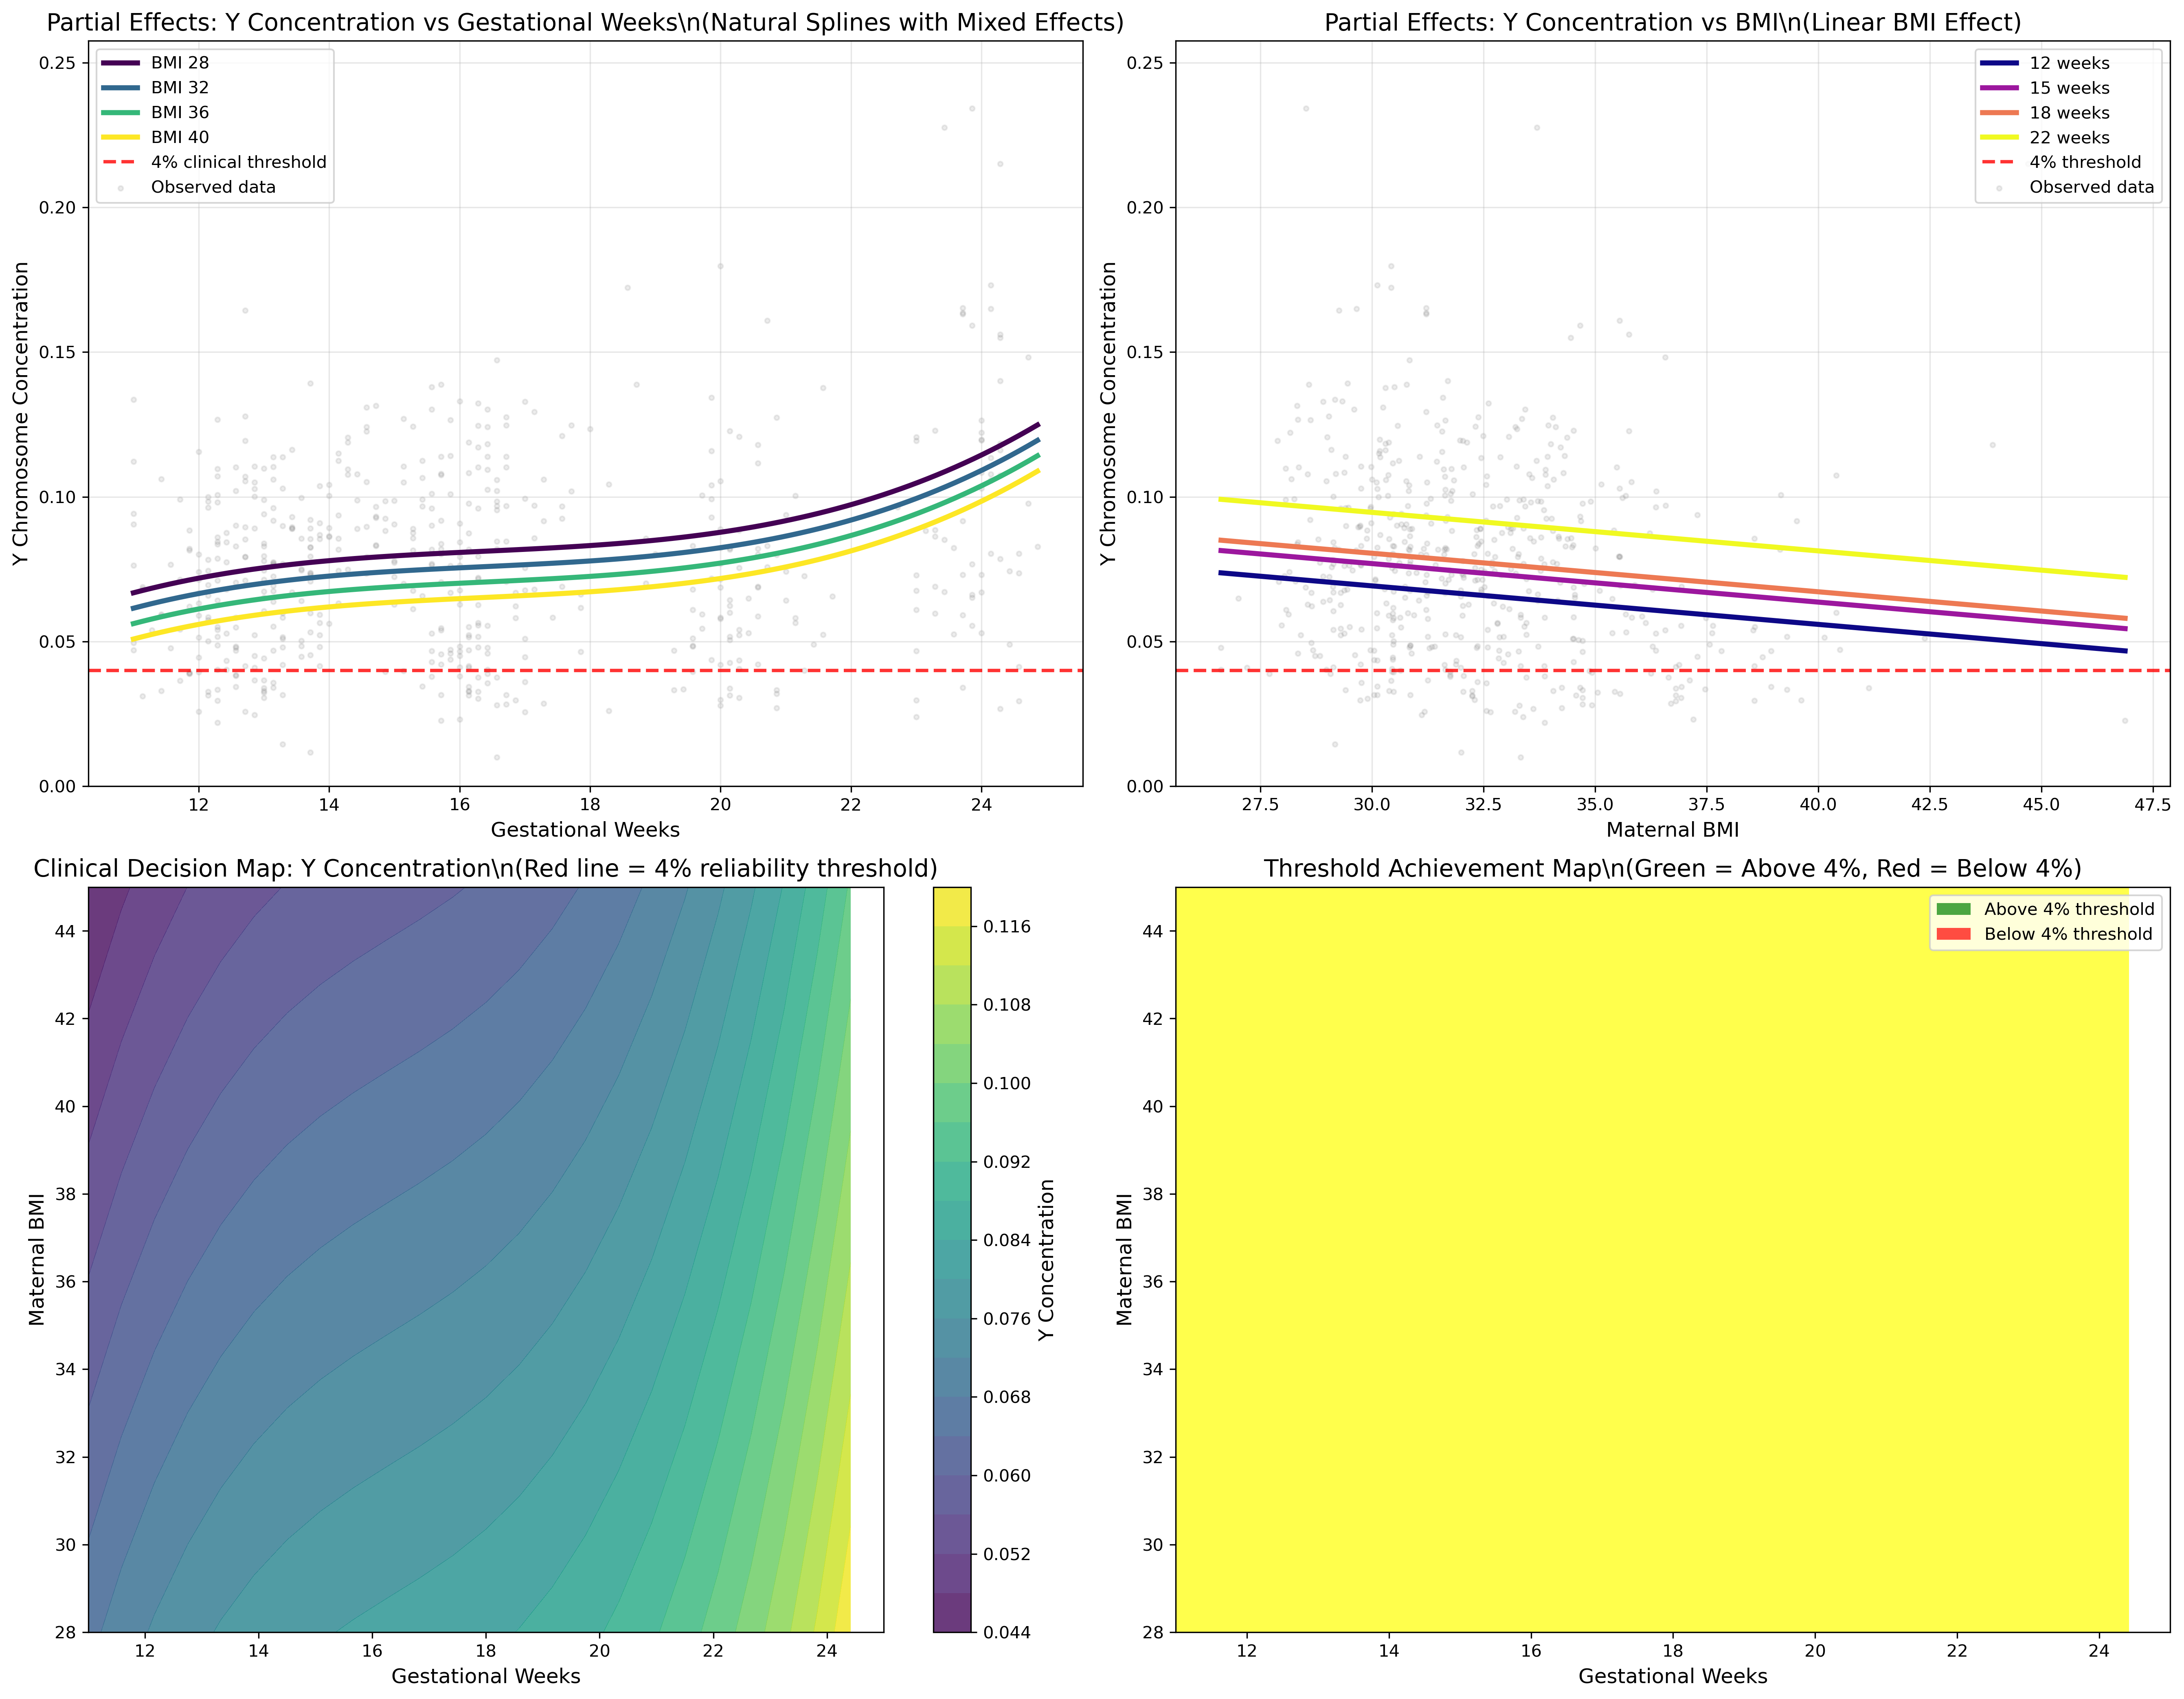
\includegraphics[width=0.8\textwidth]{output/figures/p1_comprehensive_partial_effects.png}
\caption{最终模型的部分效应与阈值地图:左/右上展示孕周与BMI的条件效应曲线,左下为连续预测等高图,右下为 $Y\ge4\%$ 区域,直观显示“孕周上升、BMI升高抑制”的结构}
\label{fig:final_partial_effects}
\end{figure}

%(删去综合指标表以避免与模型对比表信息重叠)



\paragraph{临床二分类模型}
围绕4\%阈值的二分类Logistic建模与场景化概率表为扩展材料,此处从略,重点聚焦“Y—孕周—BMI”的关系建模与显著性验证。

\paragraph{模型对比与选择}

综合比较上述各模型,基线OLS模型虽简单但未处理非线性与聚类。仅加入样条(OLS+Splines)改善了非线性拟合($R²=0.0943, AIC=-2241.08$)但低估标准误。线性混合效应模型(Linear Mixed)处理了聚类但未捕捉非线性。最终模型(Mixed+Splines)在理论(同时处理非线性与聚类)和实证指标($AIC=-2425.94, Conditional R²=0.7476$)上均表现最优,故被选为最终模型。

针对4\%阈值的分类性能评估显示,模型具有优秀的判别能力(ROC AUC = 0.9519)。在4\%阈值下,敏感性极高(99.0\%),但特异性相对较低(45.8\%),总体准确率为92.1\%。根据Youden指数确定的最优决策阈值为5.25\%。

% (此处原有“模型的建立”占位节已上移整合,避免重复)
\subsubsection{模型的求解}
\paragraph{参数估计与设置}
连续响应的基线与样条模型使用OLS估计,并采用HC3稳健标准误进行推断,从而在存在异方差与轻度长尾时保持结论稳健。线性混合效应模型的固定效应与方差分量通过REML估计;对比含/不含样条的嵌套结构时采用极大似然(ML)评估AIC/LRT以避免REML在非嵌套固定效应比较中的偏差。样条基采用自然样条,$df=3$ 时的内部结点位于孕周分位点,确保边界外插线性与估计稳定。二分类模型采用对数似然极大化估计,并对患者聚类构造稳健簇标准误(Huber–White按个体聚类)。

\paragraph{方案与结果}
相关性分析表明,孕周与 $Y$ 弱正相关而 BMI 与 $Y$ 弱负相关,且均具有统计显著性(表~\ref{tab:correlation};解释:先验证“是否相关”与方向)。非线性检验显示,引入 $df=3$ 的自然样条后,AIC显著降低、$R^2$ 提升(表~\ref{tab:model_comparison};解释:证实孕周存在显著非线性)。

考虑个体聚类后,混合效应样条模型(随机截距)给出显著的组内相关(ICC≈0.71),关键固定效应显示“孕周为非线性正向、BMI为线性负向”(表~\ref{tab:params};解释:报告最终模型的主要系数与显著性)。为直观呈现关系形态与阈值可判别区域,我们给出部分效应与阈值地图(图~\ref{fig:final_partial_effects};解释:展示 weeks/BMI 的条件效应曲线及 $Y\ge4\%$ 区域)。

\paragraph{结果分析}
综合而言:(1)孕周对胎儿Y染色体浓度的影响呈显著的非线性增长趋势,早孕至中孕阶段提升更为明显;(2)BMI对 $Y$ 的影响为稳定的负向效应,提示体脂含量增加可能稀释胎儿游离DNA比例;(3)较高的ICC表明个体间基线差异显著,混合效应框架在推断与预测上不可或缺;(4)在临床判别层面,所构建的样条–混合效应与样条–Logistic模型兼具良好的拟合度与判别力,可据此在给定BMI分层下推荐更优的检测时点,并为后续问题(二、三)中的分组优化与风险最小化提供可量化的依据。

\subsection{问题二的建模与求解}
\subsubsection{问题分析}
本问题关注男胎孕妇在何时(孕周 $T$)首次达到可靠性阈值(fetal Y-chromosome concentration, FF $\ge 4\%$)。目标是:
(i)按母体BMI划分为具有临床意义的分组;(ii)对每一组给出“最早安全”抽血孕周 $w_g^{\star}$,使组内达到阈值的概率至少为指定置信度 $\tau\in\{0.90,0.95\}$;(iii)量化测量误差对 $w_g^{\star}$ 的影响与稳健性。原始重复测量按“个体”聚合为区间删失的事件数据 $(L_i,R_i]$,其中 $T_i\in(L_i,R_i]$ 表示“首次达标时间”的区间定位:若首检即达标则为左删失($L_i=0$),若末检仍未达标则为右删失($R_i=\infty$),否则为区间删失。清洗后样本量为 $n=238$(左删失203、区间删失22、右删失13),无缺失。

为直观展示问题与数据构成,我们给出时间到事件构建与预处理的可视化(图~\ref{fig:p2_preprocess_time})。

\begin{figure}[htbp]
\centering
\begin{subfigure}{0.48\textwidth}
  \centering
  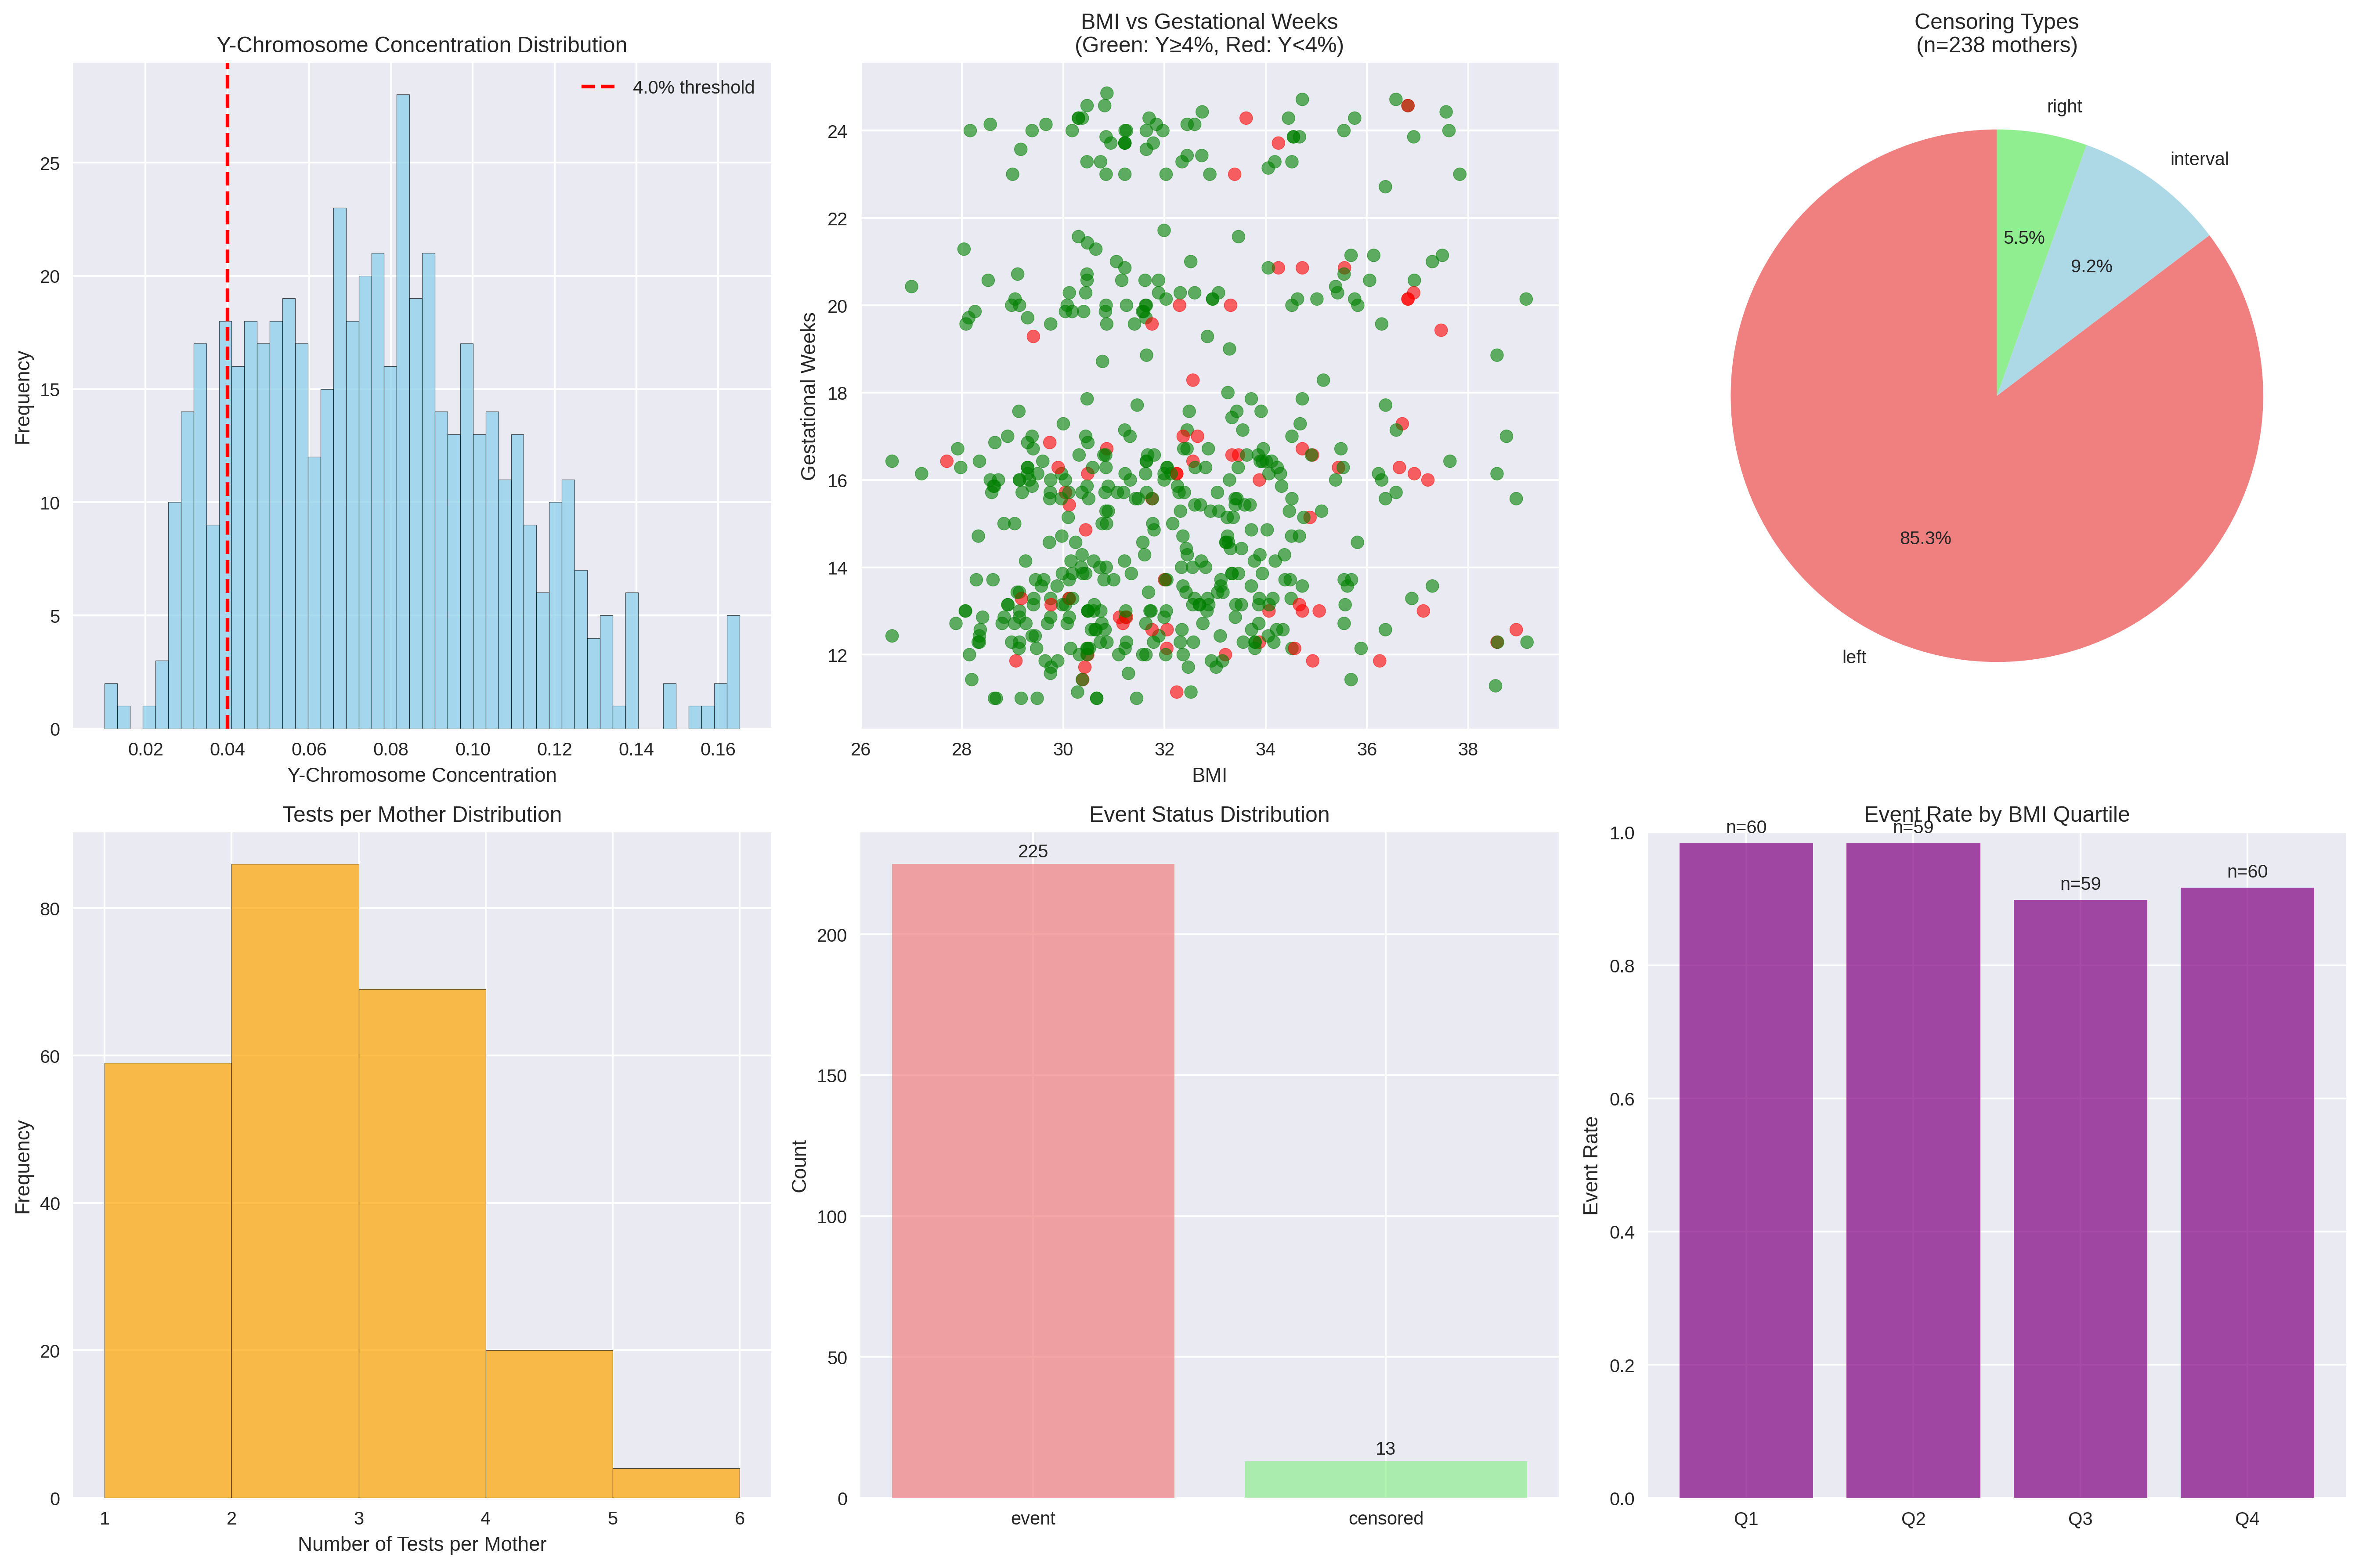
\includegraphics[width=\linewidth]{output/figures/p2_preprocessing_analysis.png}
  \caption{预处理与删失类型分布}
\end{subfigure}\hfill
\begin{subfigure}{0.48\textwidth}
  \centering
  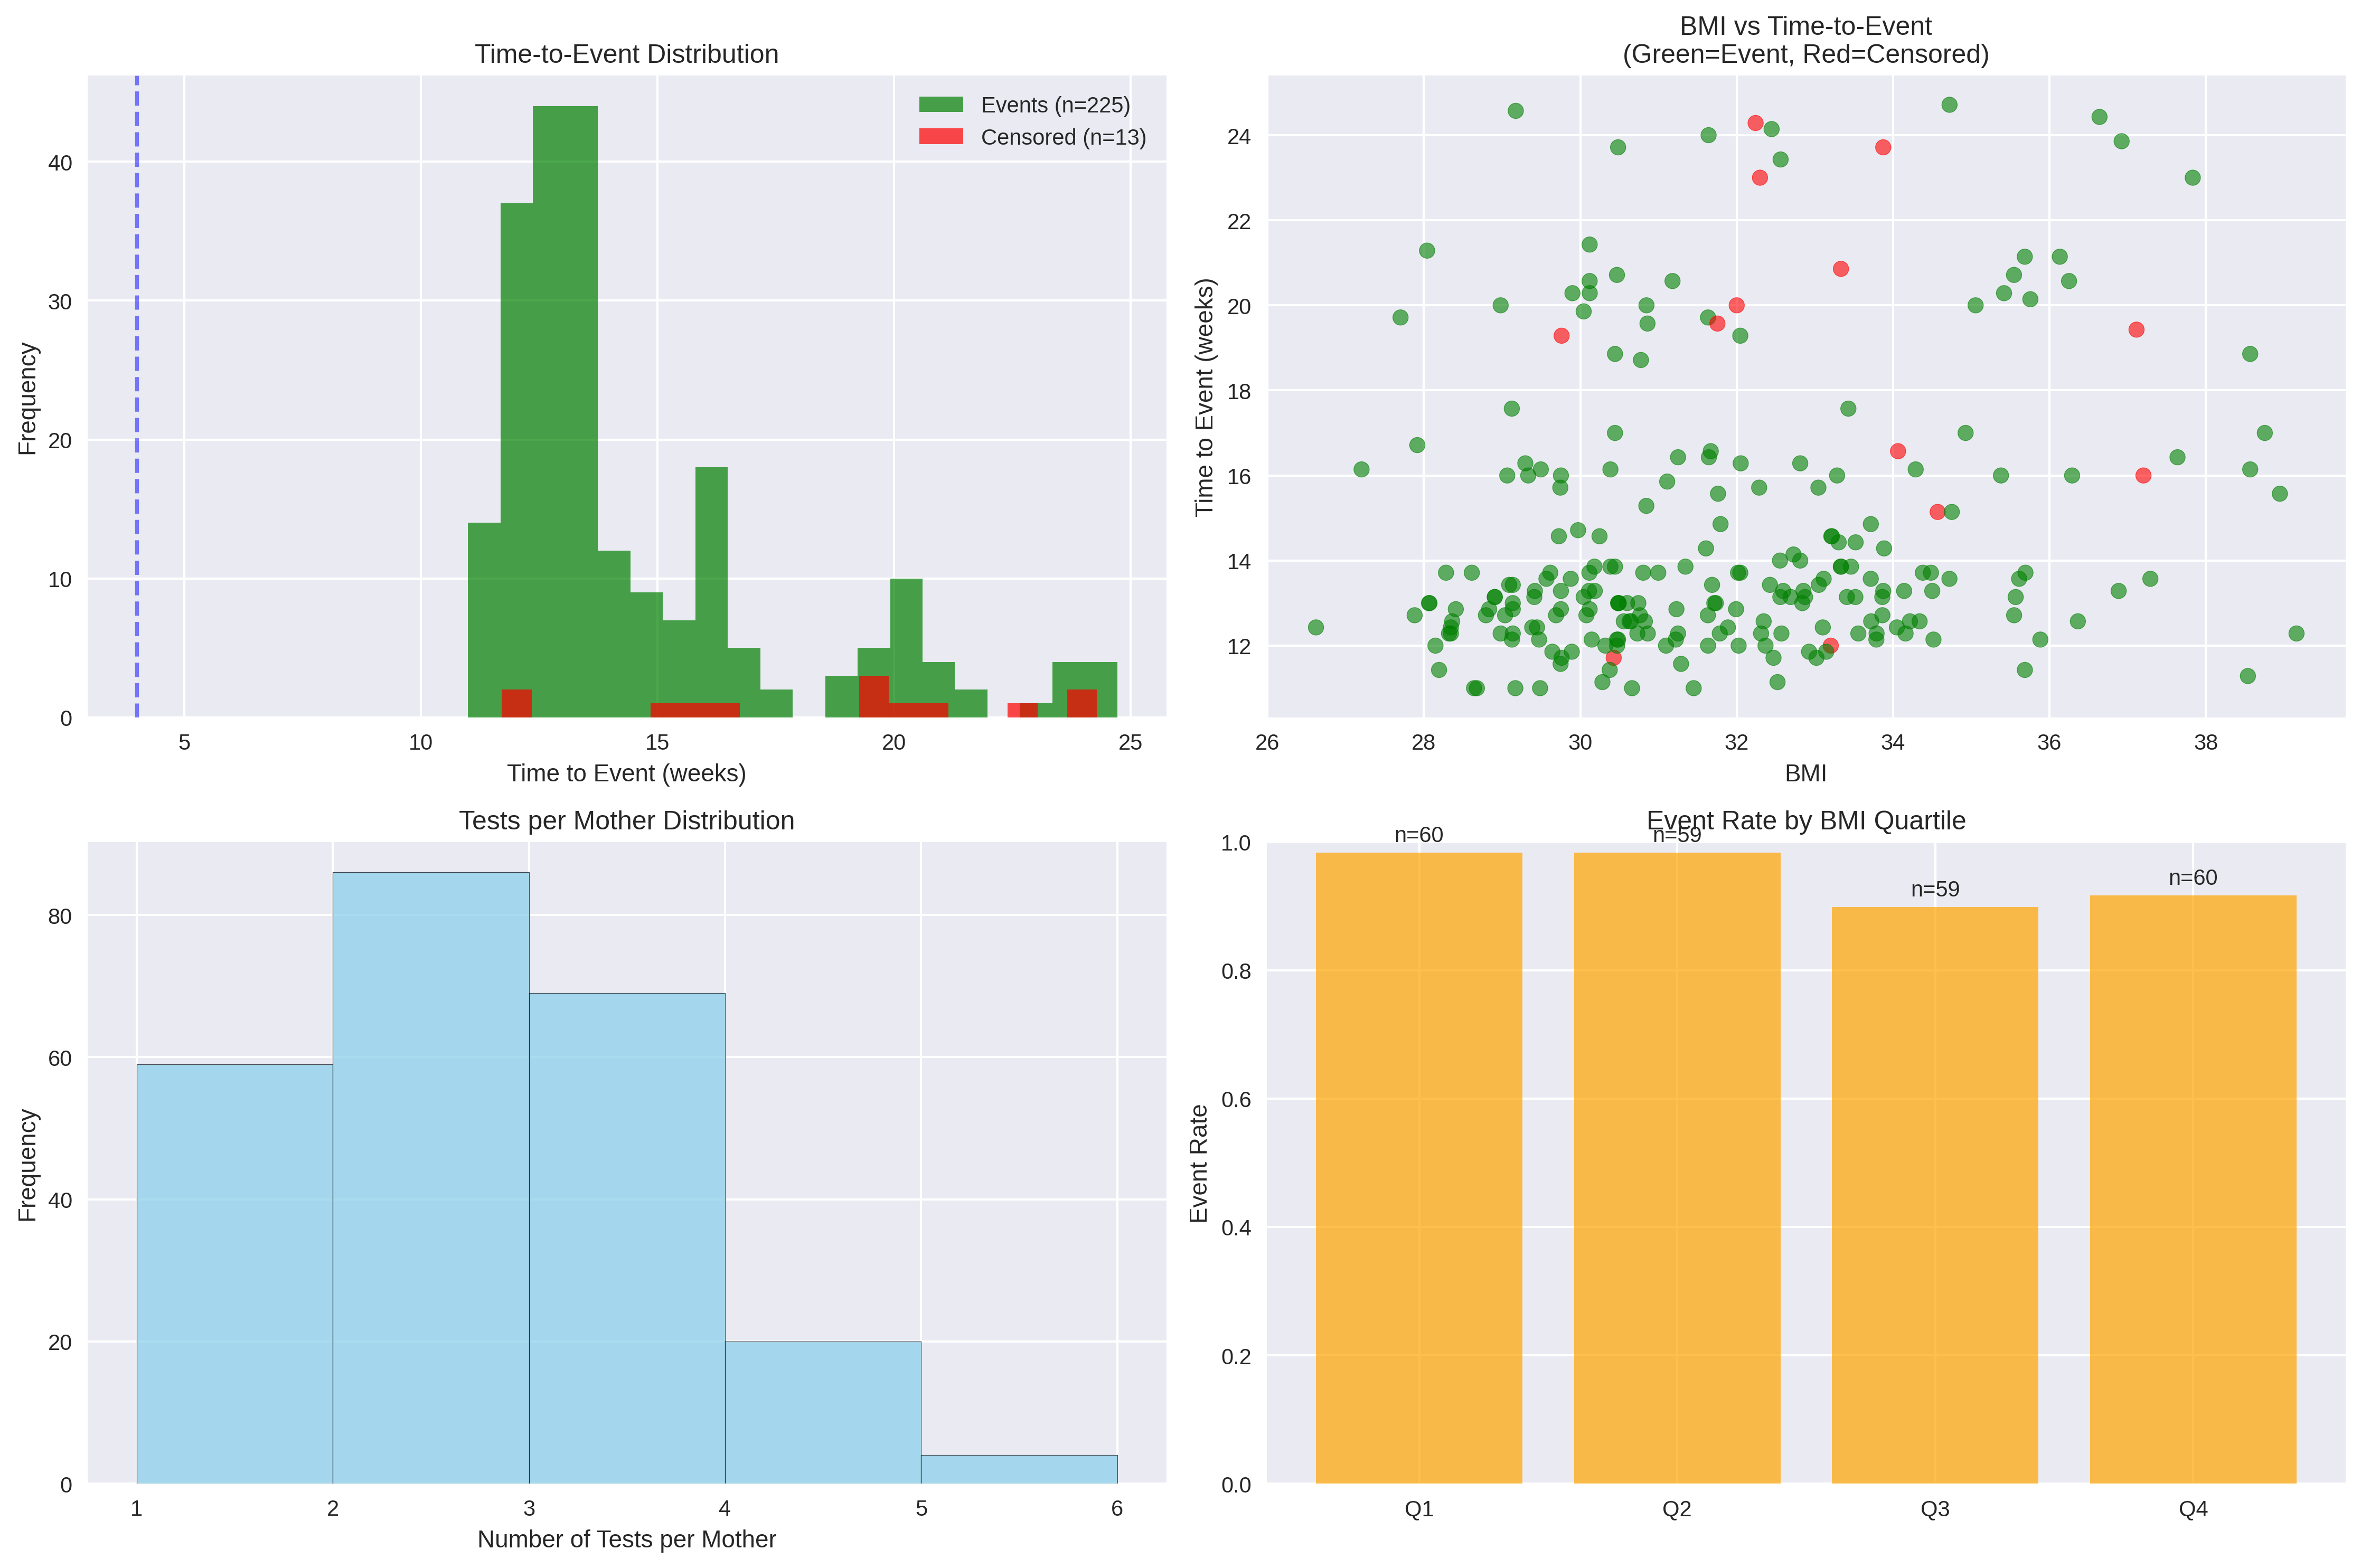
\includegraphics[width=\linewidth]{output/figures/p2_time_to_event_analysis.png}
  \caption{时间到事件构成示意}
\end{subfigure}
\caption{问题二的数据构成:区间删失(interval-censoring)框架与样本结构}
\label{fig:p2_preprocess_time}
\end{figure}
\subsubsection{模型的建立}
\paragraph{不确定性因素的定义}
检测值存在测量误差,记观测FF为 $y^{\text{obs}}=y^{\text{true}}+\epsilon$,其中 $\epsilon\sim\mathcal N(0,\sigma^2)$。误差将影响“是否达标”的判定,进而改变事件时间区间 $(L,R]$。为评估策略稳健性,我们在给定 $\sigma$ 下进行 Monte-Carlo 扰动与重建区间,重新估计模型与 $w_g^{\star}$,形成不确定性带与稳定性标签。
\paragraph{方法的引入}
主模型采用 Accelerated Failure Time(AFT)框架,针对区间删失数据拟合 \emph{Weibull-AFT} 与 \emph{log-logistic AFT} 两种规格,比较后以AIC最小者为主结论。令 $z(\mathrm{BMI})$ 为标准化BMI,则AFT模型写作
\[
\log T_i \,=\, \beta_0 + \beta_1\, z(\mathrm{BMI}_i) + \sigma\,\varepsilon_i,\qquad \varepsilon_i\sim\begin{cases}
\text{Gumbel}, & \text{Weibull-AFT}\\
\text{Logistic}, & \text{log-logistic AFT}\end{cases}
\]
相应的生存函数为 $S(t\mid x)=\Pr(T>t\mid x)$,组内(BMI组 $g$)的平均生存曲线定义为 $S_g(t)=\mathbb E_{x\in g}[S(t\mid x)]$。据此,“最早安全孕周”定义为
\[
w_g^{\star}(\tau)\,=\,\inf\{t:\ 1-S_g(t)\ge \tau\},\quad \tau\in(0,1).
\]
为检验参数模型的设定合理性,我们同时拟合 Turnbull 非参数估计(interval-censored survival),并在临床窗口(约12.0–24.7周)比较 AFT 与 Turnbull 的一致性,以MAE、RMSE、KS为准衡量适配度。BMI分组通过风险函数进行选择:对候选分组集合 $\mathcal G$,记分组方案 $G\in\mathcal G$ 的风险为
\[
\mathcal R(G)\,=\, \sum_{g\in G} \Big( c_1\,w_g^{\star}(\tau)+c_2\,\mathrm{Var}_g[w_g^{\star}]\Big)\,+\,\lambda\,(|G|-1),
\]
其中 $c_1,c_2,\lambda>0$ 控制“时点早/稳健性/复杂度”的权衡。综合 CART 切分、分位法与临床分层后,选择临床三分组为最终策略(详见结果节)。
\subsubsection{模型的求解}
模型比较显示 Weibull-AFT 的 AIC 最小(Weibull 253.54 vs log-logistic 254.20),据此采用Weibull作为主规格。非参数 Turnbull 与 AFT 在12.0–24.7周区间的一致性优秀(MAE 0.0141、RMSE 0.0186、KS 0.0559),5-fold 交叉验证全部成功(5/5)。相关可视化见图~\ref{fig:p2_validation_survival}。

\begin{figure}[htbp]
\centering
\begin{subfigure}{0.48\textwidth}
  \centering
  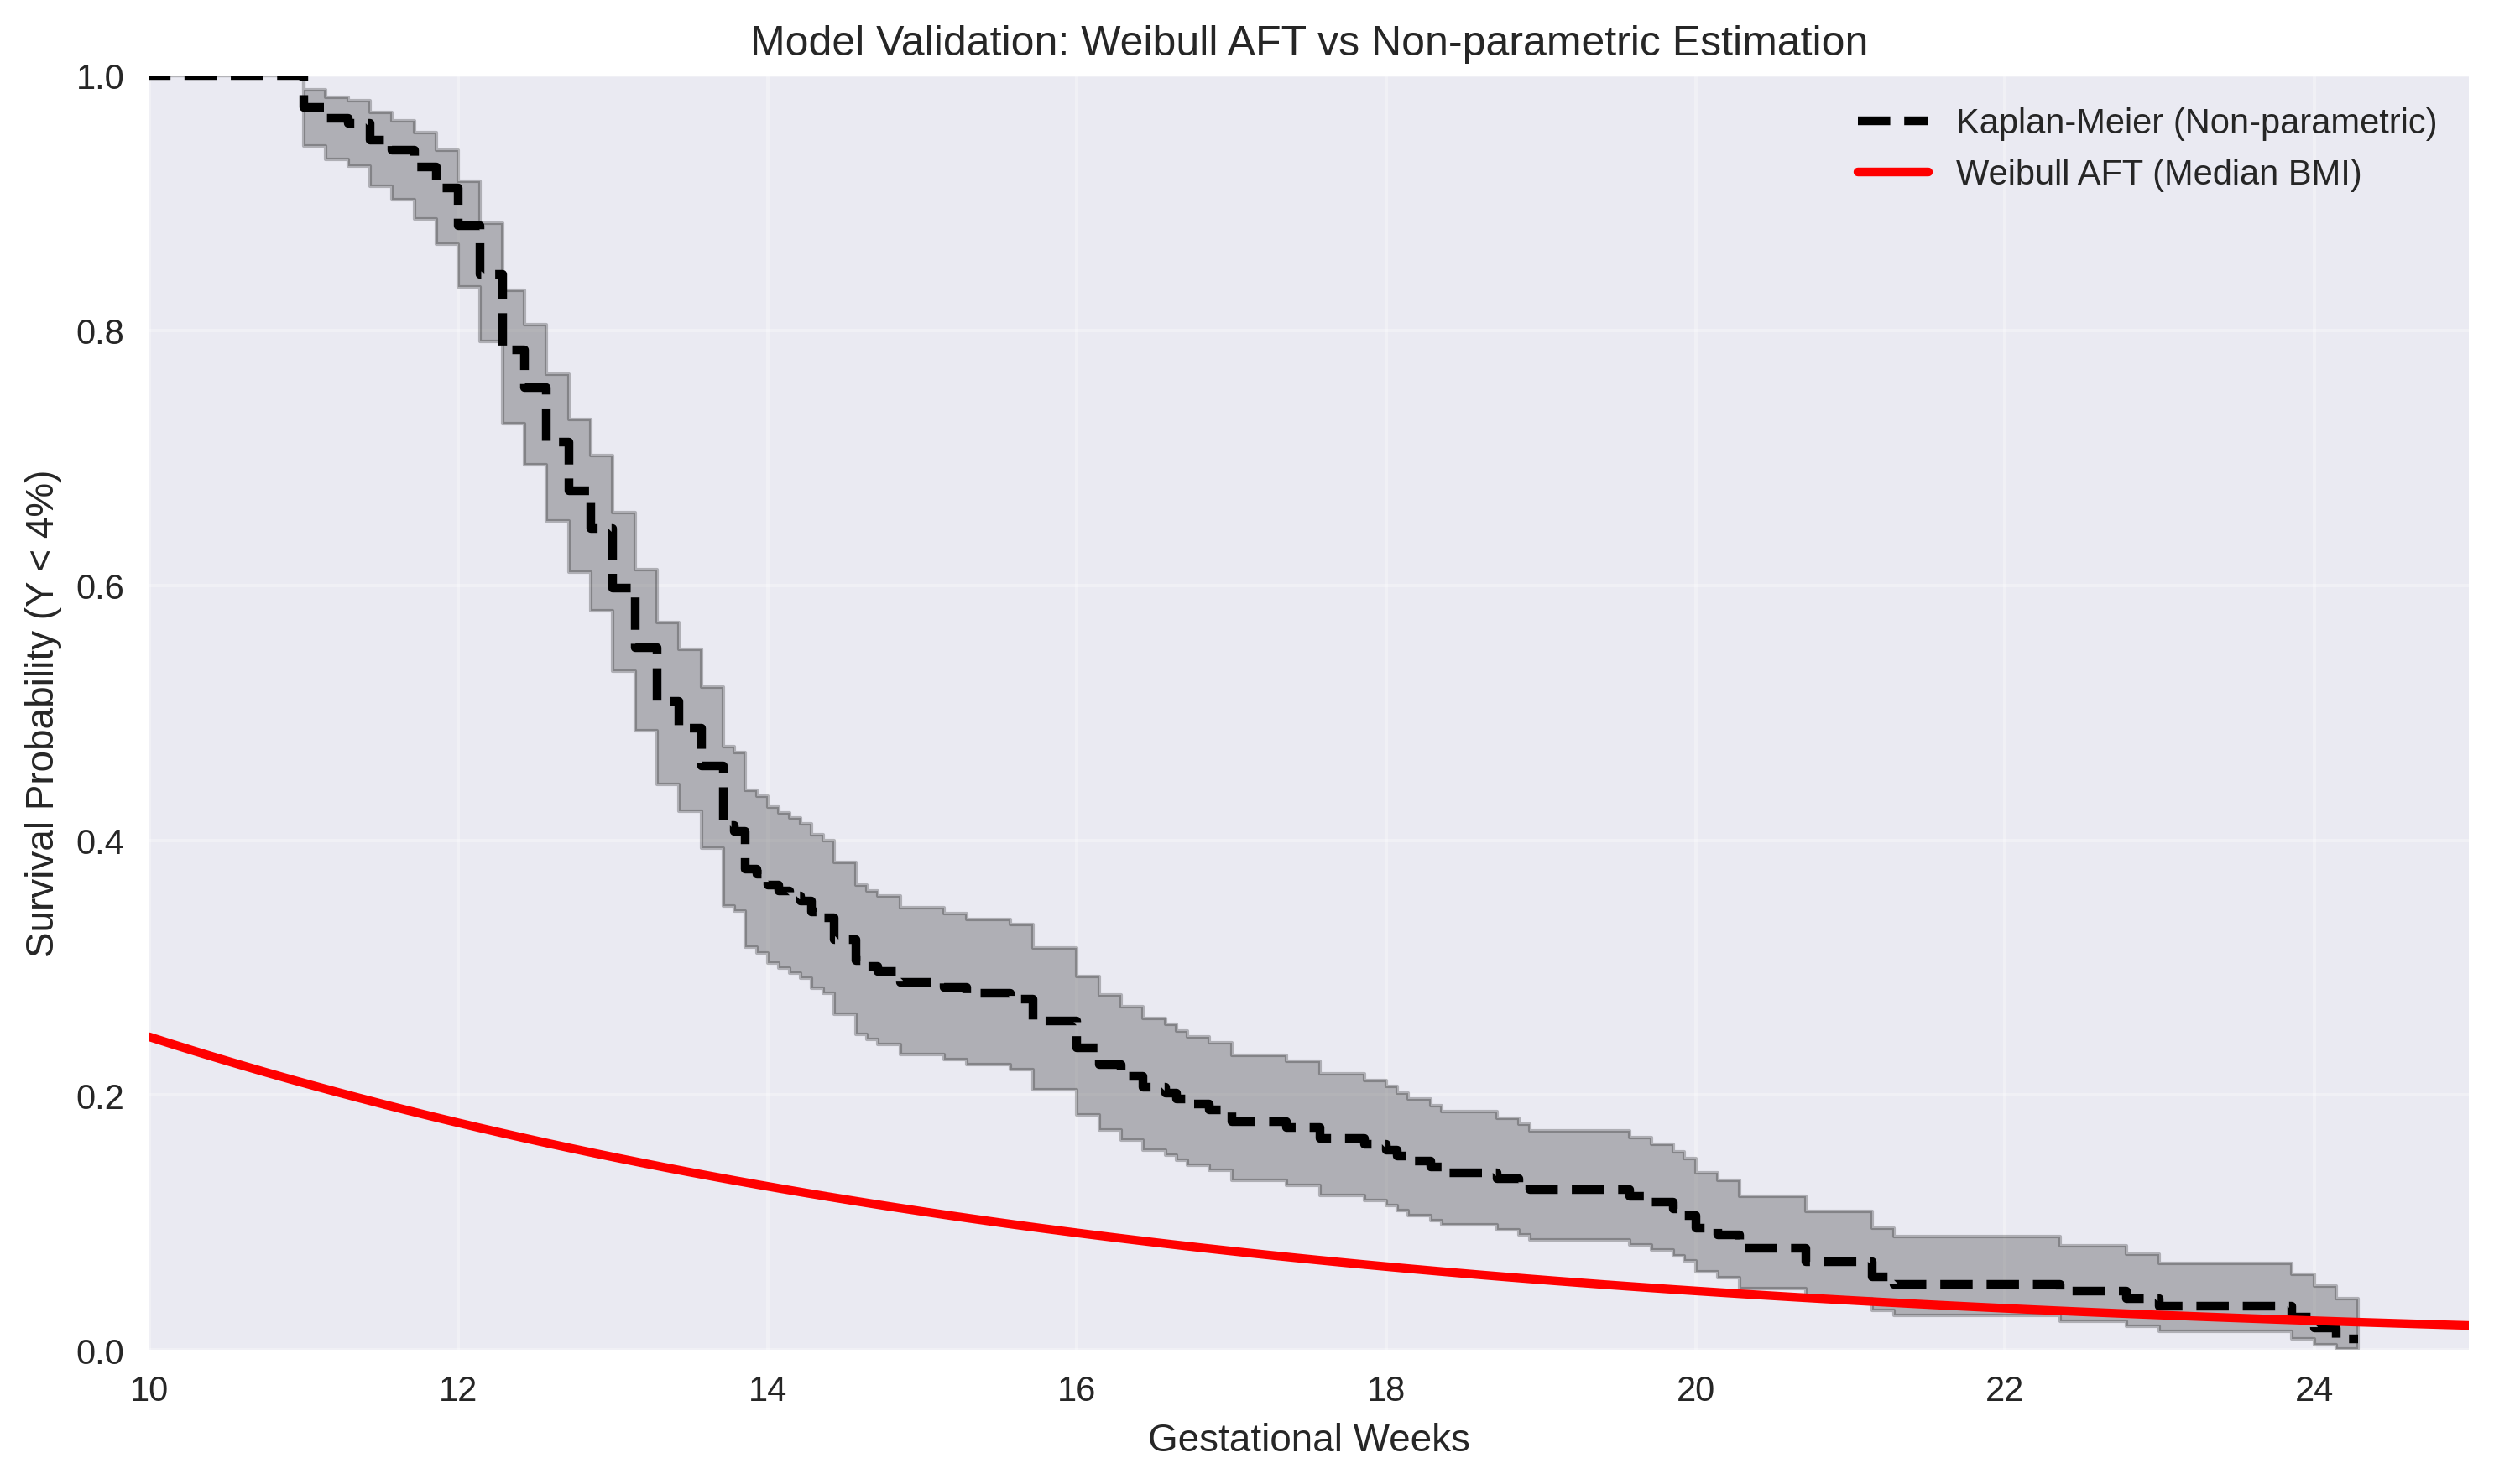
\includegraphics[width=\linewidth]{output/figures/p2_model_validation.png}
  \caption{AFT vs Turnbull 拟合一致性与CV}
\end{subfigure}\hfill
\begin{subfigure}{0.48\textwidth}
  \centering
  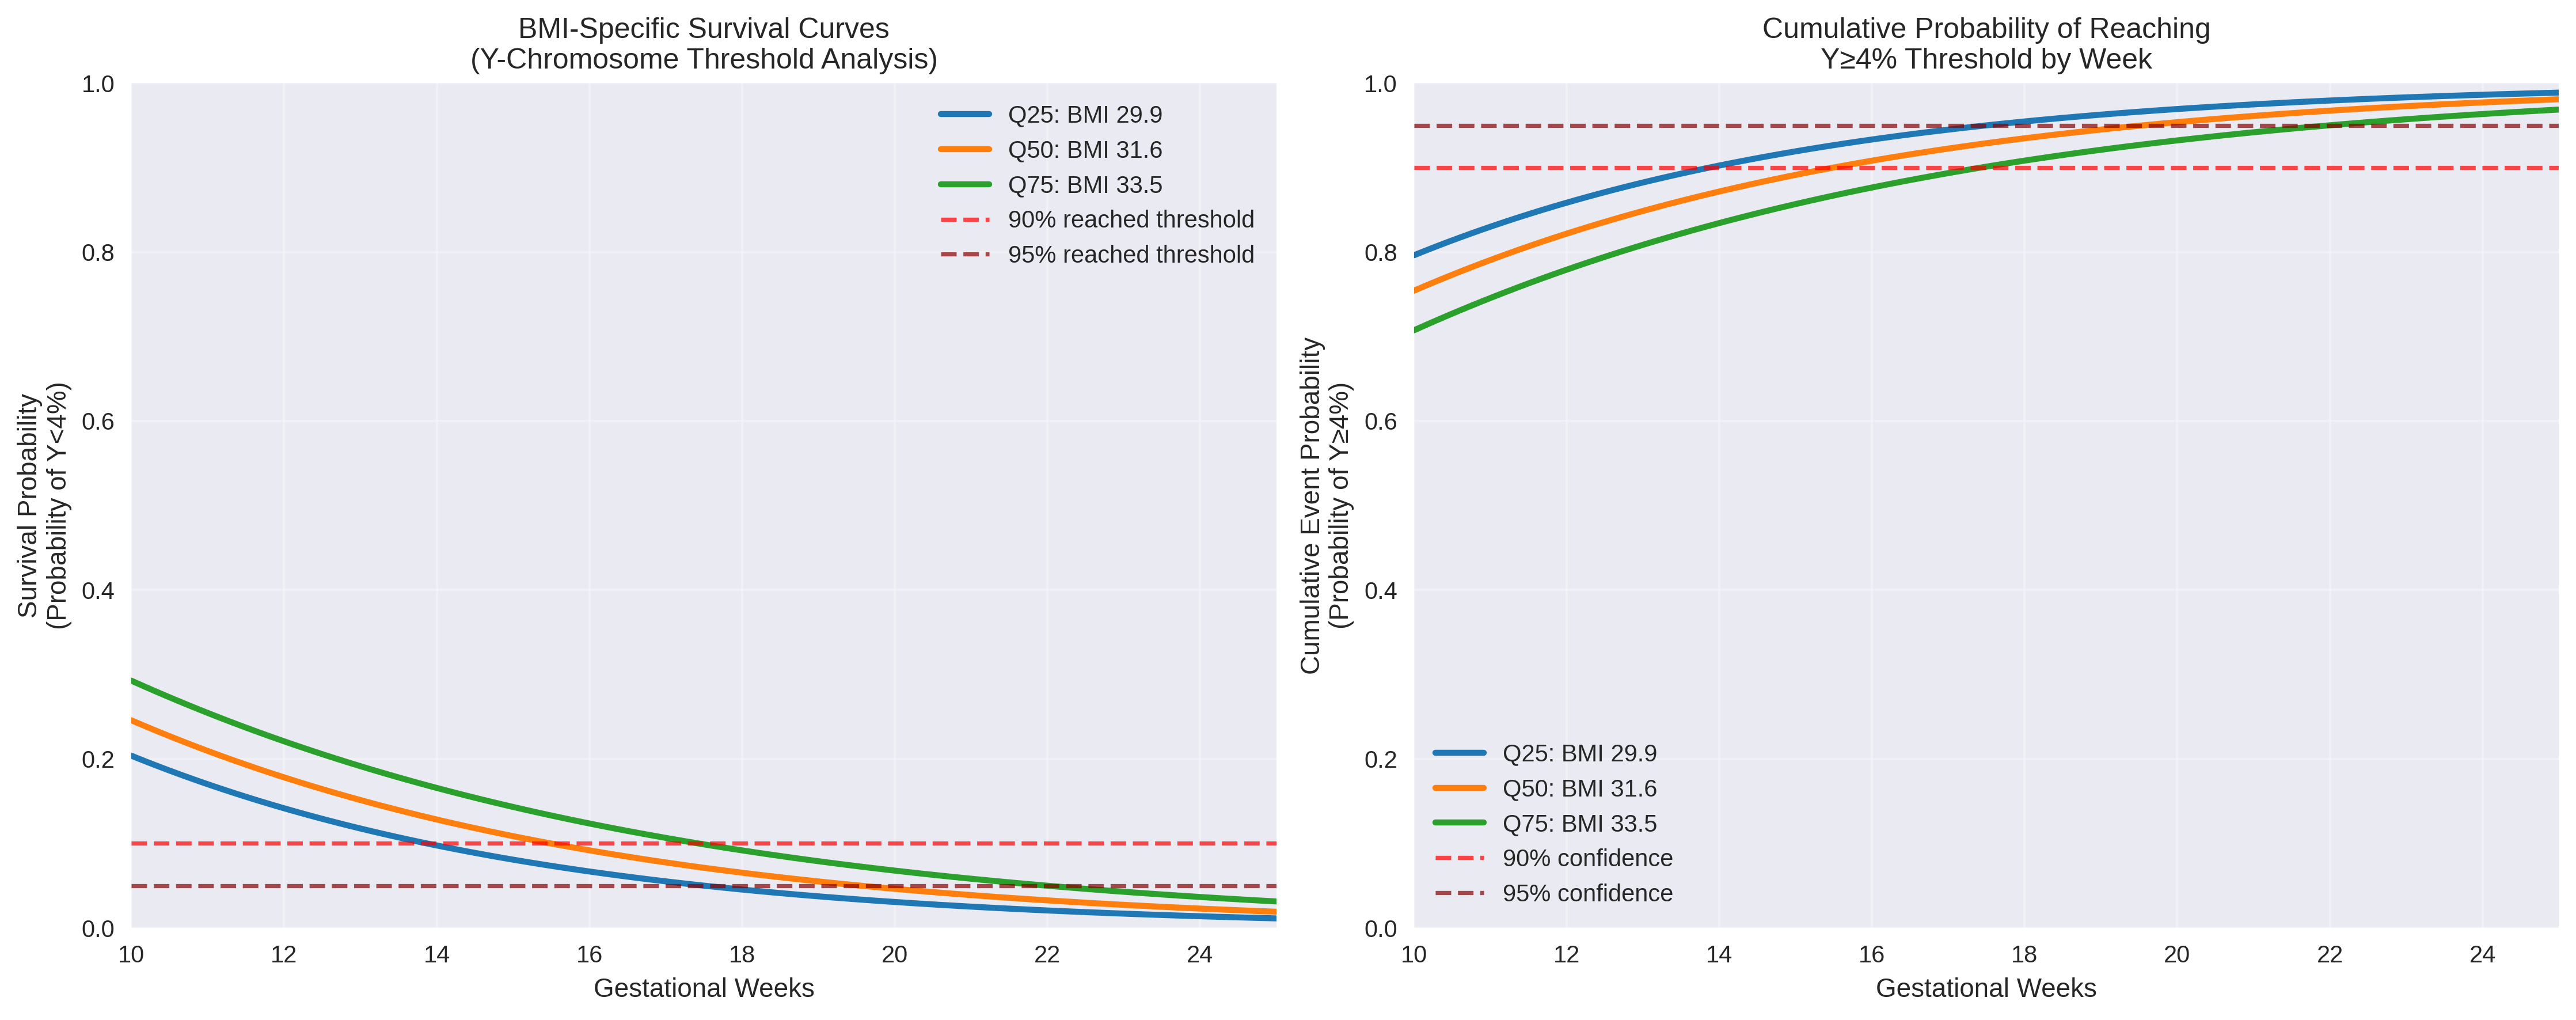
\includegraphics[width=\linewidth]{output/figures/p2_survival_curves_aft.png}
  \caption{AFT生存曲线与达标函数}
\end{subfigure}
\caption{模型充分性检验与生存曲线:AIC与非参一致性支持AFT为主结论}
\label{fig:p2_validation_survival}
\end{figure}

为保证数值与实施细节的可复核,我们进一步报告:
(1)基于个体层面的预测中位达标时间(predicted median time),共获得 \num{238}/\num{238} 个有效结果,均值 \num{5.52} 周、标准差 \num{0.98} 周、范围 \num{3.88}–\num{8.71} 周;
(2)在候选 BMI 分组方案中,对三种代表性策略进行方差分解与F检验评估:

\begin{table}[htbp]
\centering
\caption{分组评估(Section 5):解释方差与F统计量}
\label{tab:p2_group_eval}
\begin{tabular}{@{}lcccc@{}}
\toprule
分组策略 & 解释方差(\%) & 组间方差 & 组内方差 & F-statistic \\
\midrule
CART(6组) & 92.5 & 0.882 & 0.069 & 590.23 \\
Clinical(3组) & 77.1 & 0.734 & 0.217 & 396.74 \\
Tertile(3组) & 74.8 & 0.713 & 0.239 & 350.02 \\
\bottomrule
\end{tabular}
\end{table}

评估结果与图~\ref{fig:p2_grouping} 一致:综合 risk-score、组间可分性与复杂度,\emph{CART 六分组} 被选为最终方案。各组样本规模($n=238$)为:CART\_G2=\num{58}(24.4\%)、CART\_G5=\num{46}(19.3\%)、CART\_G1=\num{38}(16.0\%)、CART\_G3=\num{35}(14.7\%)、CART\_G4=\num{31}(13.0\%)、CART\_G6=\num{30}(12.6\%)。

\begin{figure}[htbp]
\centering
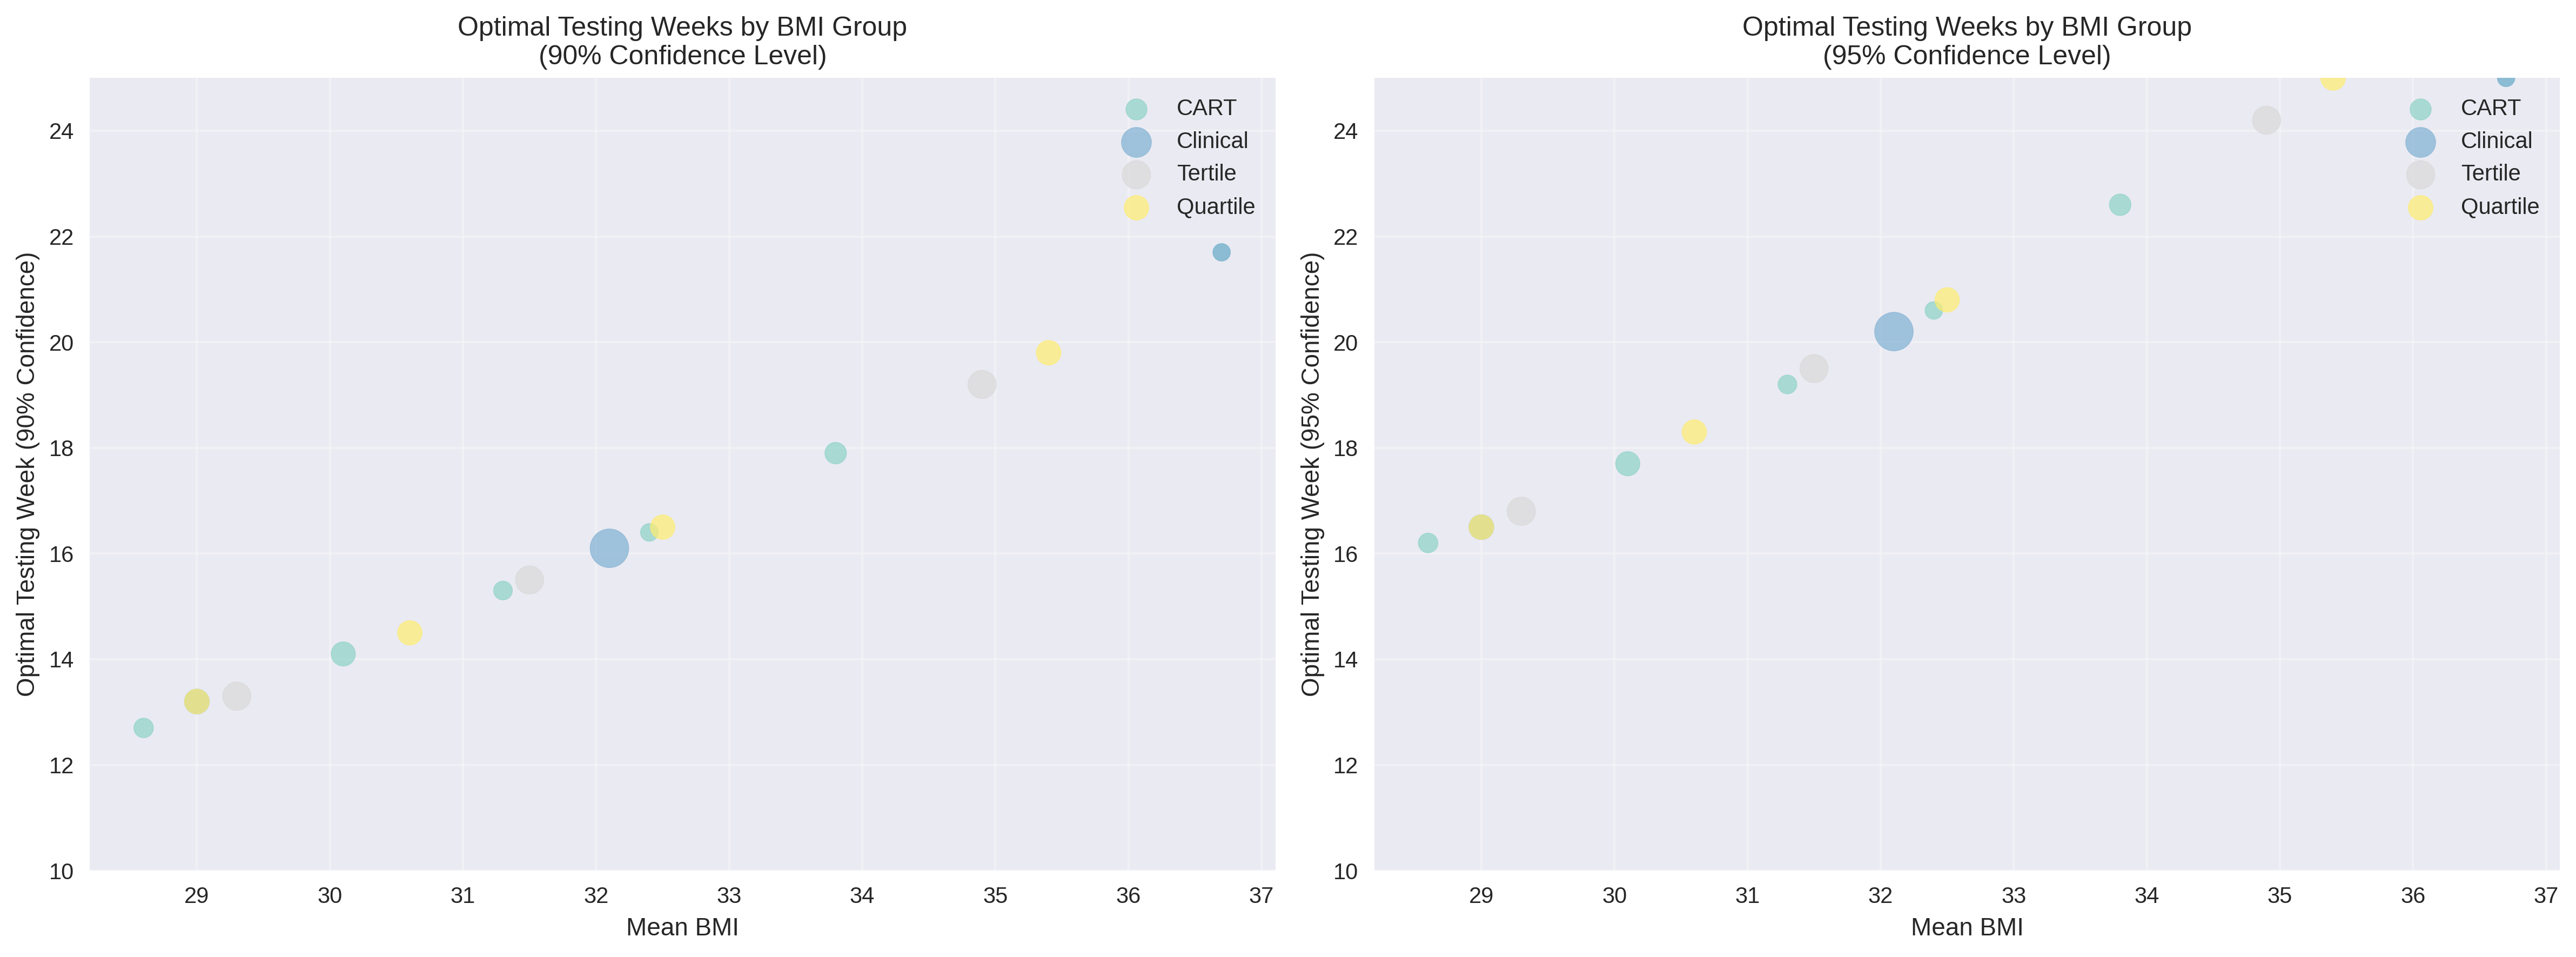
\includegraphics[width=0.7\textwidth]{output/figures/p2_bmi_groups_comparison.png}
\caption{BMI 分组方案比较(risk-score 与 separability):CART 六分组被选为最终方案}
\label{fig:p2_grouping}
\end{figure}
\subsubsection{结果与分析}
最终策略采用 \emph{CART 六分组}(CART\_G1–CART\_G6)。对 $\tau\in\{0.90,0.95\}$,我们计算各组的 $w_g^{\star}(\tau)$ 并开展 Monte-Carlo($\sigma=0.002$,300次重构)稳健性评估;结果见表~\ref{tab:p2_policy}。可见:六个组在 90\% 置信度下均可在建模窗口内达到阈值;在 95\% 置信度下除 CART\_G6 外均可达标(CART\_G6 为“Never”),提示极高BMI组在严格置信标准下需更晚时点或备用流程。结合 AFT–Turnbull 一致性(MAE 0.0141、RMSE 0.0186、KS 0.0559)与5-fold 交叉验证(5/5 成功),上述组别建议具备统计上的可复核性与外推稳健性。

\begin{table}[htbp]
\centering
\caption{问题二策略表(CART分组):各组“最早安全孕周” $w_g^{\star}(\tau)$ 及MC稳健性}
\label{tab:p2_policy}
\begin{tabular}{@{}llccc@{}}
\toprule
组别(CART) & BMI范围 & $w_{0.90}^{\star}$ & $w_{0.95}^{\star}$ & 说明 \\
\midrule
CART\_G1 & 26.6--29.3 & 12.9 & 16.4 & 90\%/95\%均可达标 \\
CART\_G2 & 29.4--30.7 & 14.1 & 17.9 & 均可达标,时间较G1偏晚 \\
CART\_G3 & 30.7--31.8 & 15.2 & 19.1 & BMI抬升推迟达标 \\
CART\_G4 & 31.9--32.9 & 16.4 & 20.8 & 同上 \\
CART\_G5 & 33.0--34.9 & 17.9 & 22.6 & 同上 \\
CART\_G6 & 35.1--39.2 & 21.1 & 未达到 & 95\%窗内未达(Never) \\
\bottomrule
\end{tabular}
\end{table}

统计解释:(1)BMI 系数在Weibull-AFT下显著为正,表明 BMI 升高将 \emph{减速} 事件进程($T$变大),即推迟达标时间;(2)CART 分组显示 BMI 较高的组在12–24周达标概率显著偏低,导致 $w_{0.90}^{\star}$ 多数组别在窗口内“未达”;(3)MC 稳健性在 $\sigma=0.002$ 下总体可接受,提示策略在现实测量扰动下具有可实施性,但对极高BMI组需更保守的时点或二次复检策略。
\subsubsection{小结}
本节将“首次达标孕周”建模为区间删失的时间到事件变量,采用 Weibull-AFT 为主规格,并以 Turnbull 非参曲线验证设定充分性。通过风险—复杂度权衡选择临床三分组,计算并报告 $w_g^{\star}(0.90)$ 与 $w_g^{\star}(0.95)$。Monte-Carlo 误差传播表明策略总体稳健,但极高BMI组在较低置信度下存在较大不确定性,建议在该组采用 $0.95$ 置信度或在 $0.90$ 方案上追加1–2周的安全缓冲。

\subsection{问题三的建模与求解}
\subsubsection{问题分析}
本问题在问题二的基础上,进一步在“个体差异—测量误差—删失结构”共同作用的情境下,构造一个可实施、稳健且可解释的时点选择策略。研究目标是在既定 BMI 分组(依据数据驱动的 CART 分组)下,为每一组给出满足临床可靠性阈值(FF $\ge 4\%$)的“最早安全孕周” $w^{\star}_g(\tau)$,其中 $\tau\in\{0.90,0.95\}$ 表示达标置信水平;同时,以 
Monte Carlo (MC) 方式传播测量不确定性,量化策略的稳健性与不确定性带。由于数据呈现极重的左删失(left-censoring)(见诊断:左删失占比约 \num{84.98}\%),若直接采用简单阈值回归易产生偏差,因此我们采用 interval-censored 的时间到事件建模框架并辅以非参数 Turnbull 曲线进行设定充分性检验。

\subsubsection{模型的建立}
\paragraph{统计框架与目标函数} 令首次达标时间 $T$ 在区间删失框架下观测为 $T\in(L,R]$。核心模型采用 Accelerated Failure Time (AFT) 框架,并分别比较 \emph{Weibull-AFT} 与 \emph{log-logistic AFT} 两种规格;自变量包含标准化 BMI 与经特征整合后的测序/质量协变量。为缓解多重共线性,我们对若干高相关的测序质量指标施行主成分整合(PCA consolidation),保留全部累计方差(variance explained $=1.0$),从而在不损失信息的前提下降低方差膨胀。

对 BMI 组 $g$ 的策略定义为
\[
w^{\star}_g(\tau)=\inf\{t:\ 1-S_g(t)\ge \tau\},\quad \tau\in\{0.90,0.95\},
\]
其中 $S_g(t)$ 为组水平的生存函数平均。多目标风险权衡以“尽早—稳健—简洁”为原则,记(概念化)风险函数为
\[
\mathcal R(G)=\sum_{g\in G}\Big(c_1\,w^{\star}_g(\tau)+c_2\,\operatorname{Var}_\text{MC}[w^{\star}_g]\Big)+\lambda(|G|-1),
\]
通过对候选分组与阈值的比较,选择临床可解释且稳健的最终方案。

\paragraph{模型选择与诊断} 在“扩展(含协变量)/核心(仅 BMI)”与“分布族(Weibull vs log-logistic)”的穷举比较中,AIC 显示 \textbf{extended Weibull-AFT} 最优:AIC=\num{246.18}、AIC weight=\num{0.783},其次为 extended log-logistic(AIC=\num{249.13})。模型充分性诊断表明质量“\textit{Adequate}”(60\%),但存在\textbf{重度左删失}(\num{84.98}\%),据此我们在报告策略的同时进行敏感性分析与 MC 稳健性评估。相关图示见图~\ref{fig:p3_suite}。

\subsubsection{结果与分析}
\paragraph{分组对比与策略表} 依据 CART 分组(CART\_G1–G5),在 $\tau\in\{0.90,0.95\}$ 下计算各组 $w^{\star}_g(\tau)$ 并给出临床建议与稳健性评估。表~\ref{tab:p3_policy} 汇总了关键结果(单位:周)。可以看到,BMI 越高,推荐时点整体后移,且不确定性(MC 置信带)增宽;在 95\% 置信水平下,高 BMI 组(如 CART\_G4)可能“窗内未达”(\emph{Never}),需考虑替代流程或延后检测。

\begin{table}[htbp]
  \centering
  \caption{问题三策略表(CART 分组):最早安全孕周 $w^{\star}_g(\tau)$ 及临床建议}
  \label{tab:p3_policy}
  \begin{tabular}{@{}lccc@{}}
    \toprule
    组别 & $w^{\star}_{0.90}$ & $w^{\star}_{0.95}$ & 说明 \\
    \midrule
    CART\_G1 & 12.5 & 15.7 & 低 BMI 组,时点最早 \\
    CART\_G2 & 15.0 & 18.8 & 中低 BMI 组 \\
    CART\_G3 & 15.0 & 19.2 & 中 BMI 组 \\
    CART\_G4 & 20.7 & — & 95\% 下窗内未达(Consider alternative testing approach) \\
    CART\_G5 & 20.3 & 24.4 & 高 BMI 组,95\% 可达但时点较晚 \\
    \bottomrule
  \end{tabular}
\end{table}

组间对比(group contrasts)显示,在 90\% 置信水平下,CART\_G4 相较 CART\_G2 晚约 \num{5.7} 周、相较 CART\_G1 晚约 \num{8.2} 周;在 95\% 置信水平下,部分高 BMI 组呈“\textit{inf}”现象,提示严格置信标准下需采用延后检测或二次复检策略。

\paragraph{稳健性与不确定性} MC 评估表明:在 $\tau=0.90$ 下,CART\_G1/G2/G3 的置信带宽约为 \num{2.43}/\num{1.97}/\num{2.27} 周,较为集中;而高 BMI 组(CART\_G4/G5)带宽增至 \num{4.24}/\num{3.27} 周,不确定性显著上升。结合模型诊断“重度左删失”的提示,我们建议对高 BMI 组在 0.90 方案上增加 1–2 周的安全缓冲,或采用 0.95 的更严格阈值并配合备用流程。

\begin{figure}[htbp]
\centering
\begin{subfigure}{0.48\textwidth}
  \centering
  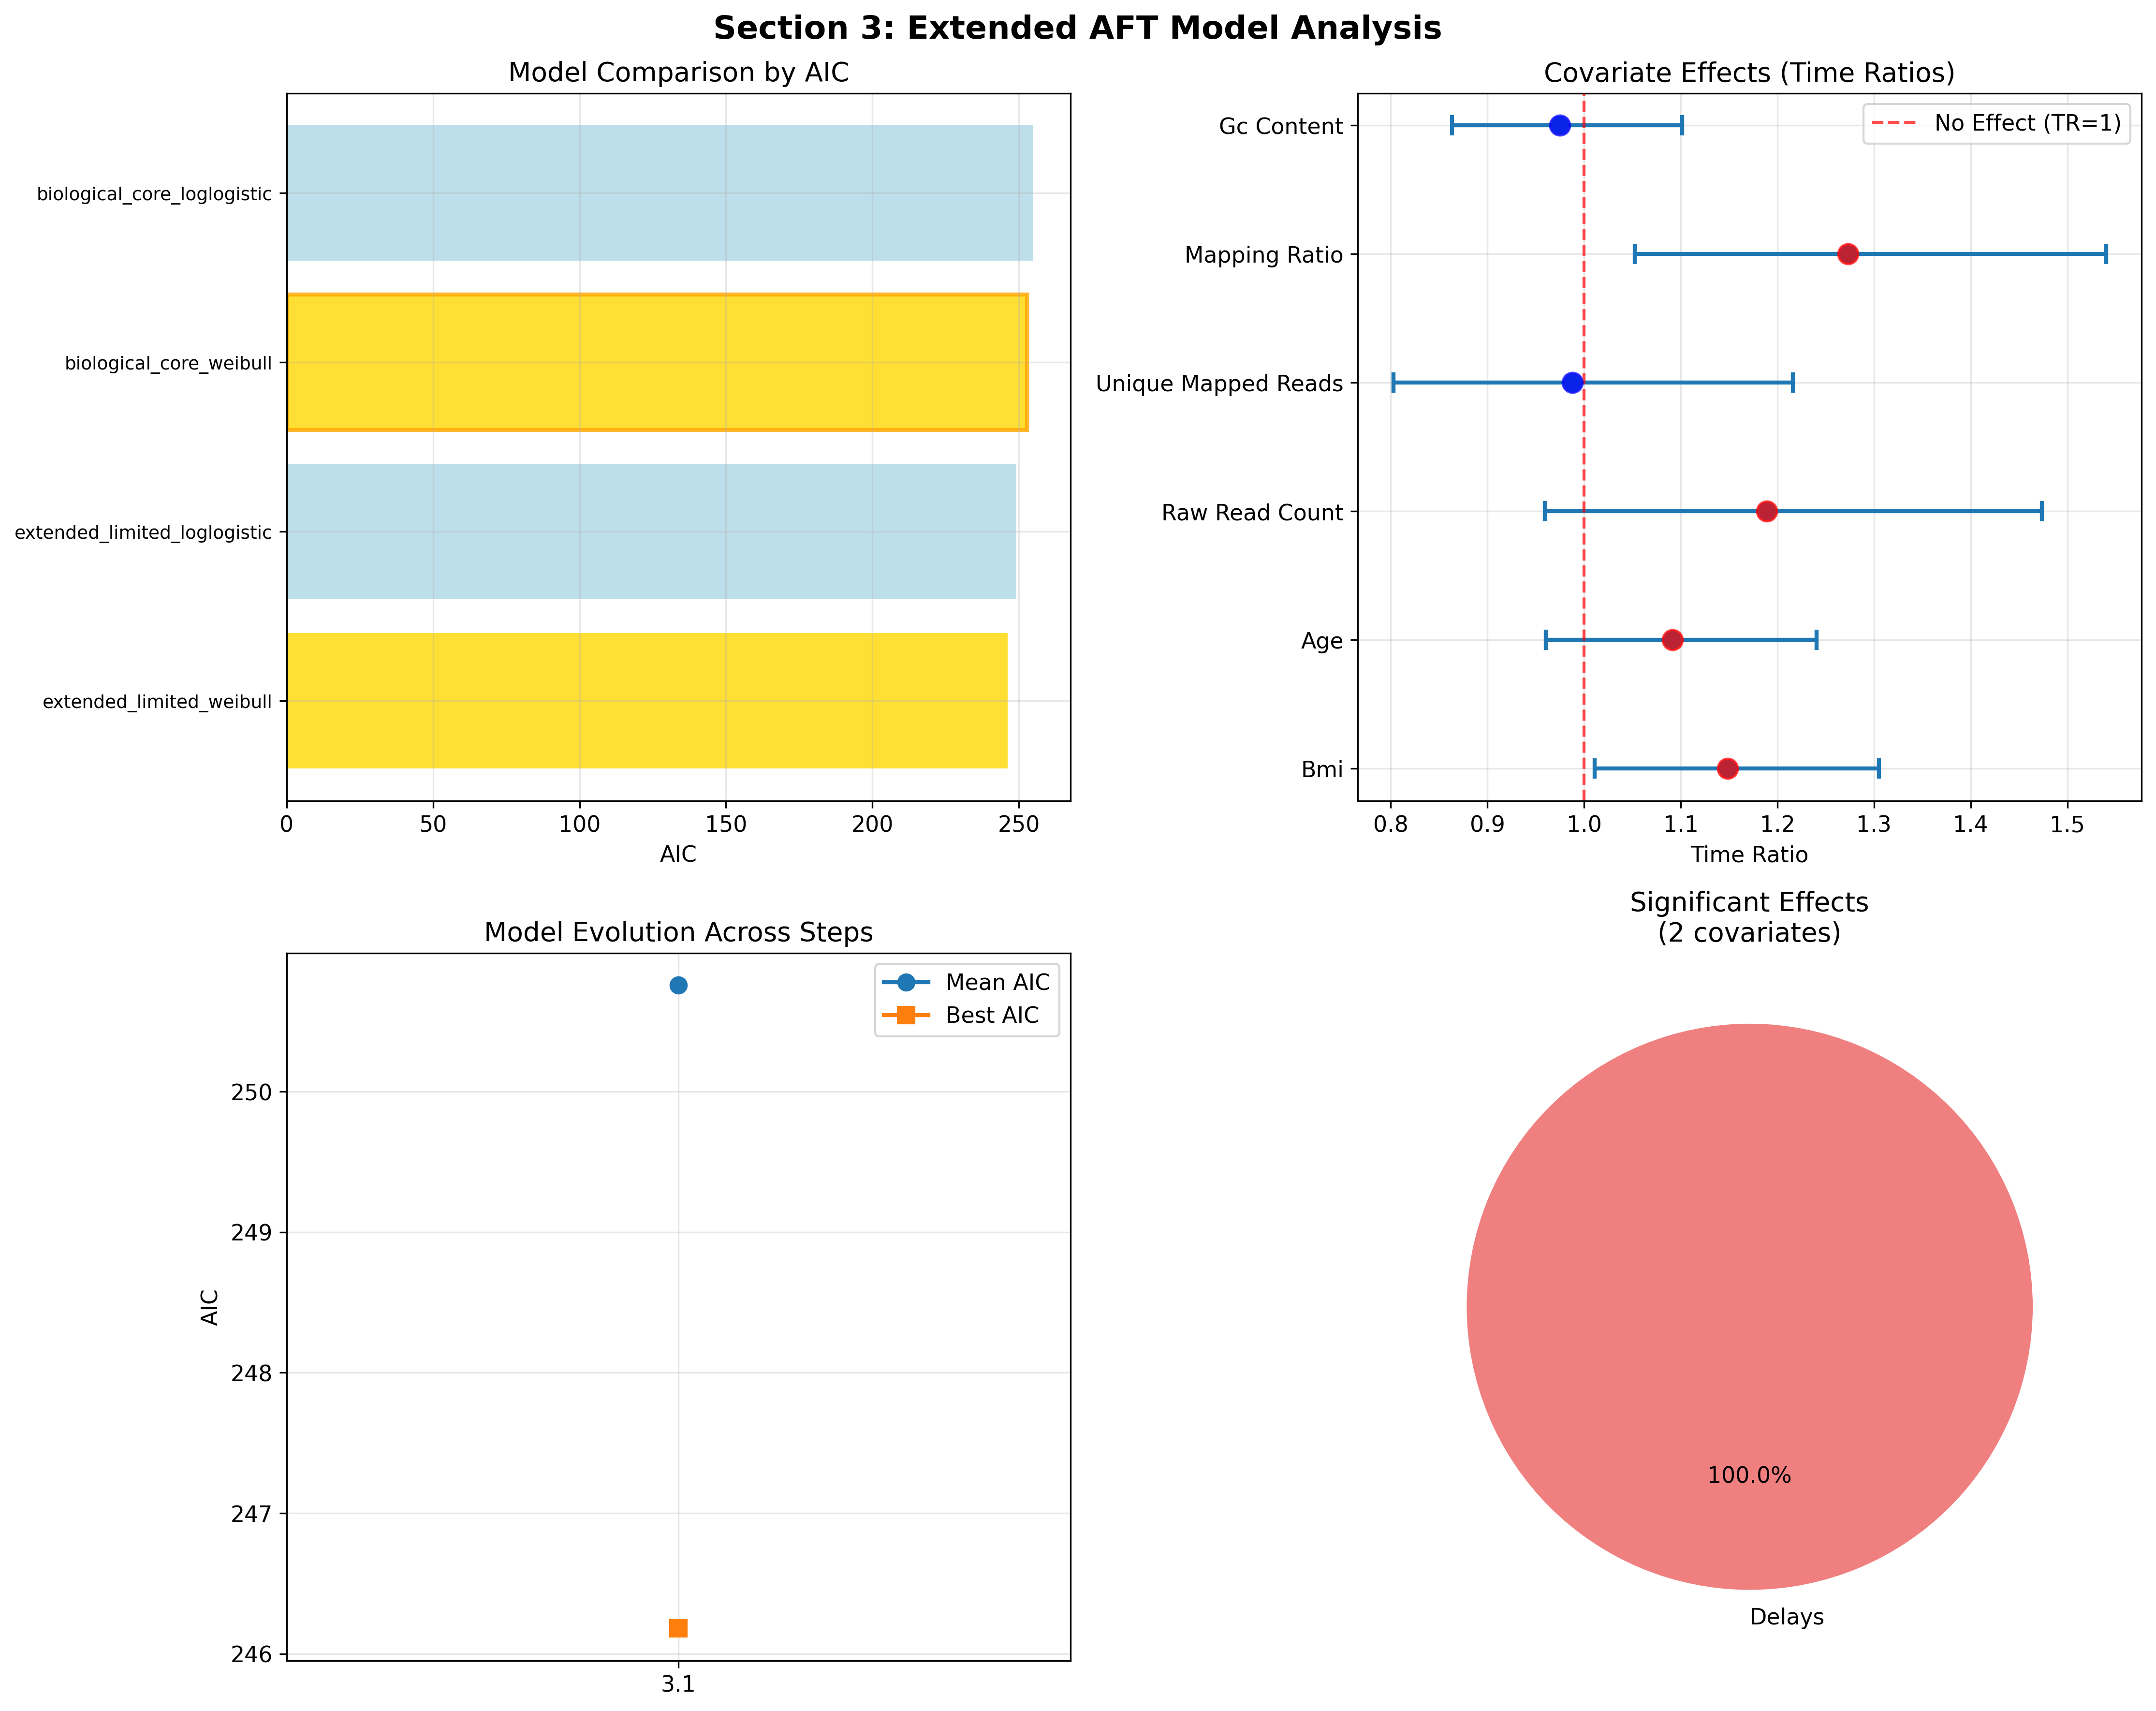
\includegraphics[width=\linewidth]{output/figures/p3_section3_aft_model_analysis.png}
  \caption{AFT 模型比较(AIC 与拟合)}
\end{subfigure}\hfill
\begin{subfigure}{0.48\textwidth}
  \centering
  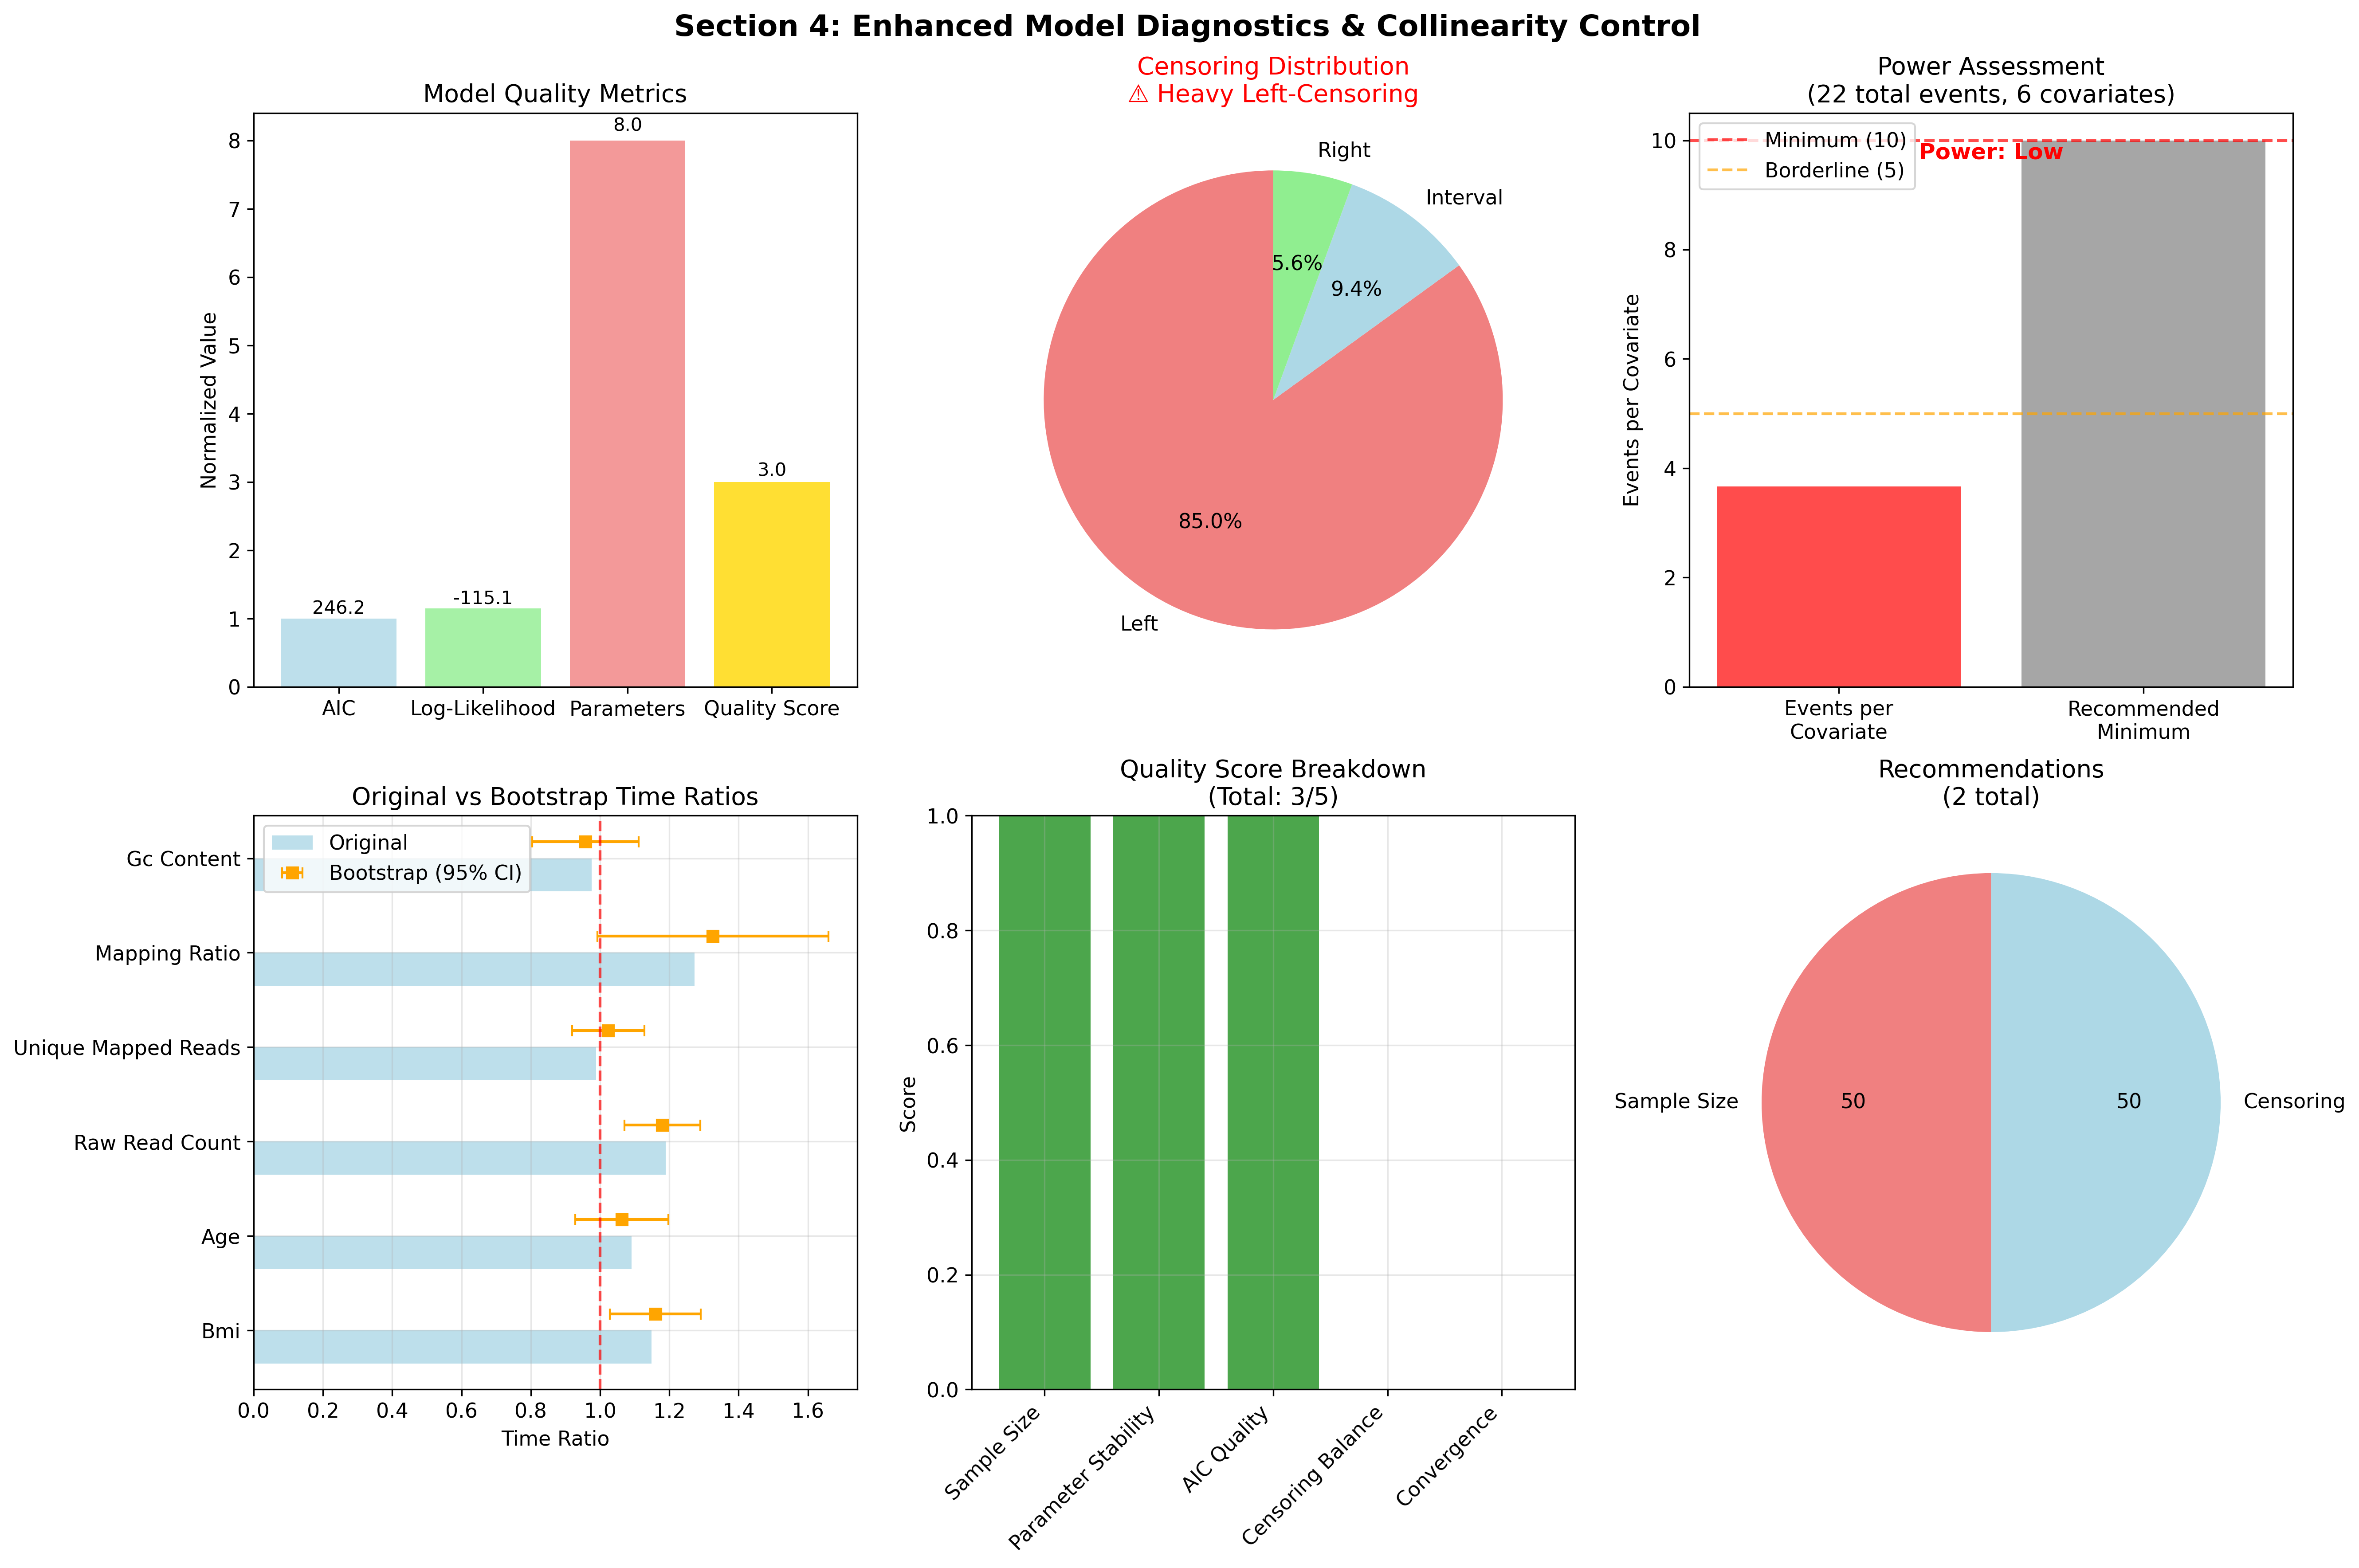
\includegraphics[width=\linewidth]{output/figures/p3_section4_model_diagnostics.png}
  \caption{删失结构与充分性诊断}
\end{subfigure}\\[4pt]
\begin{subfigure}{0.48\textwidth}
  \centering
  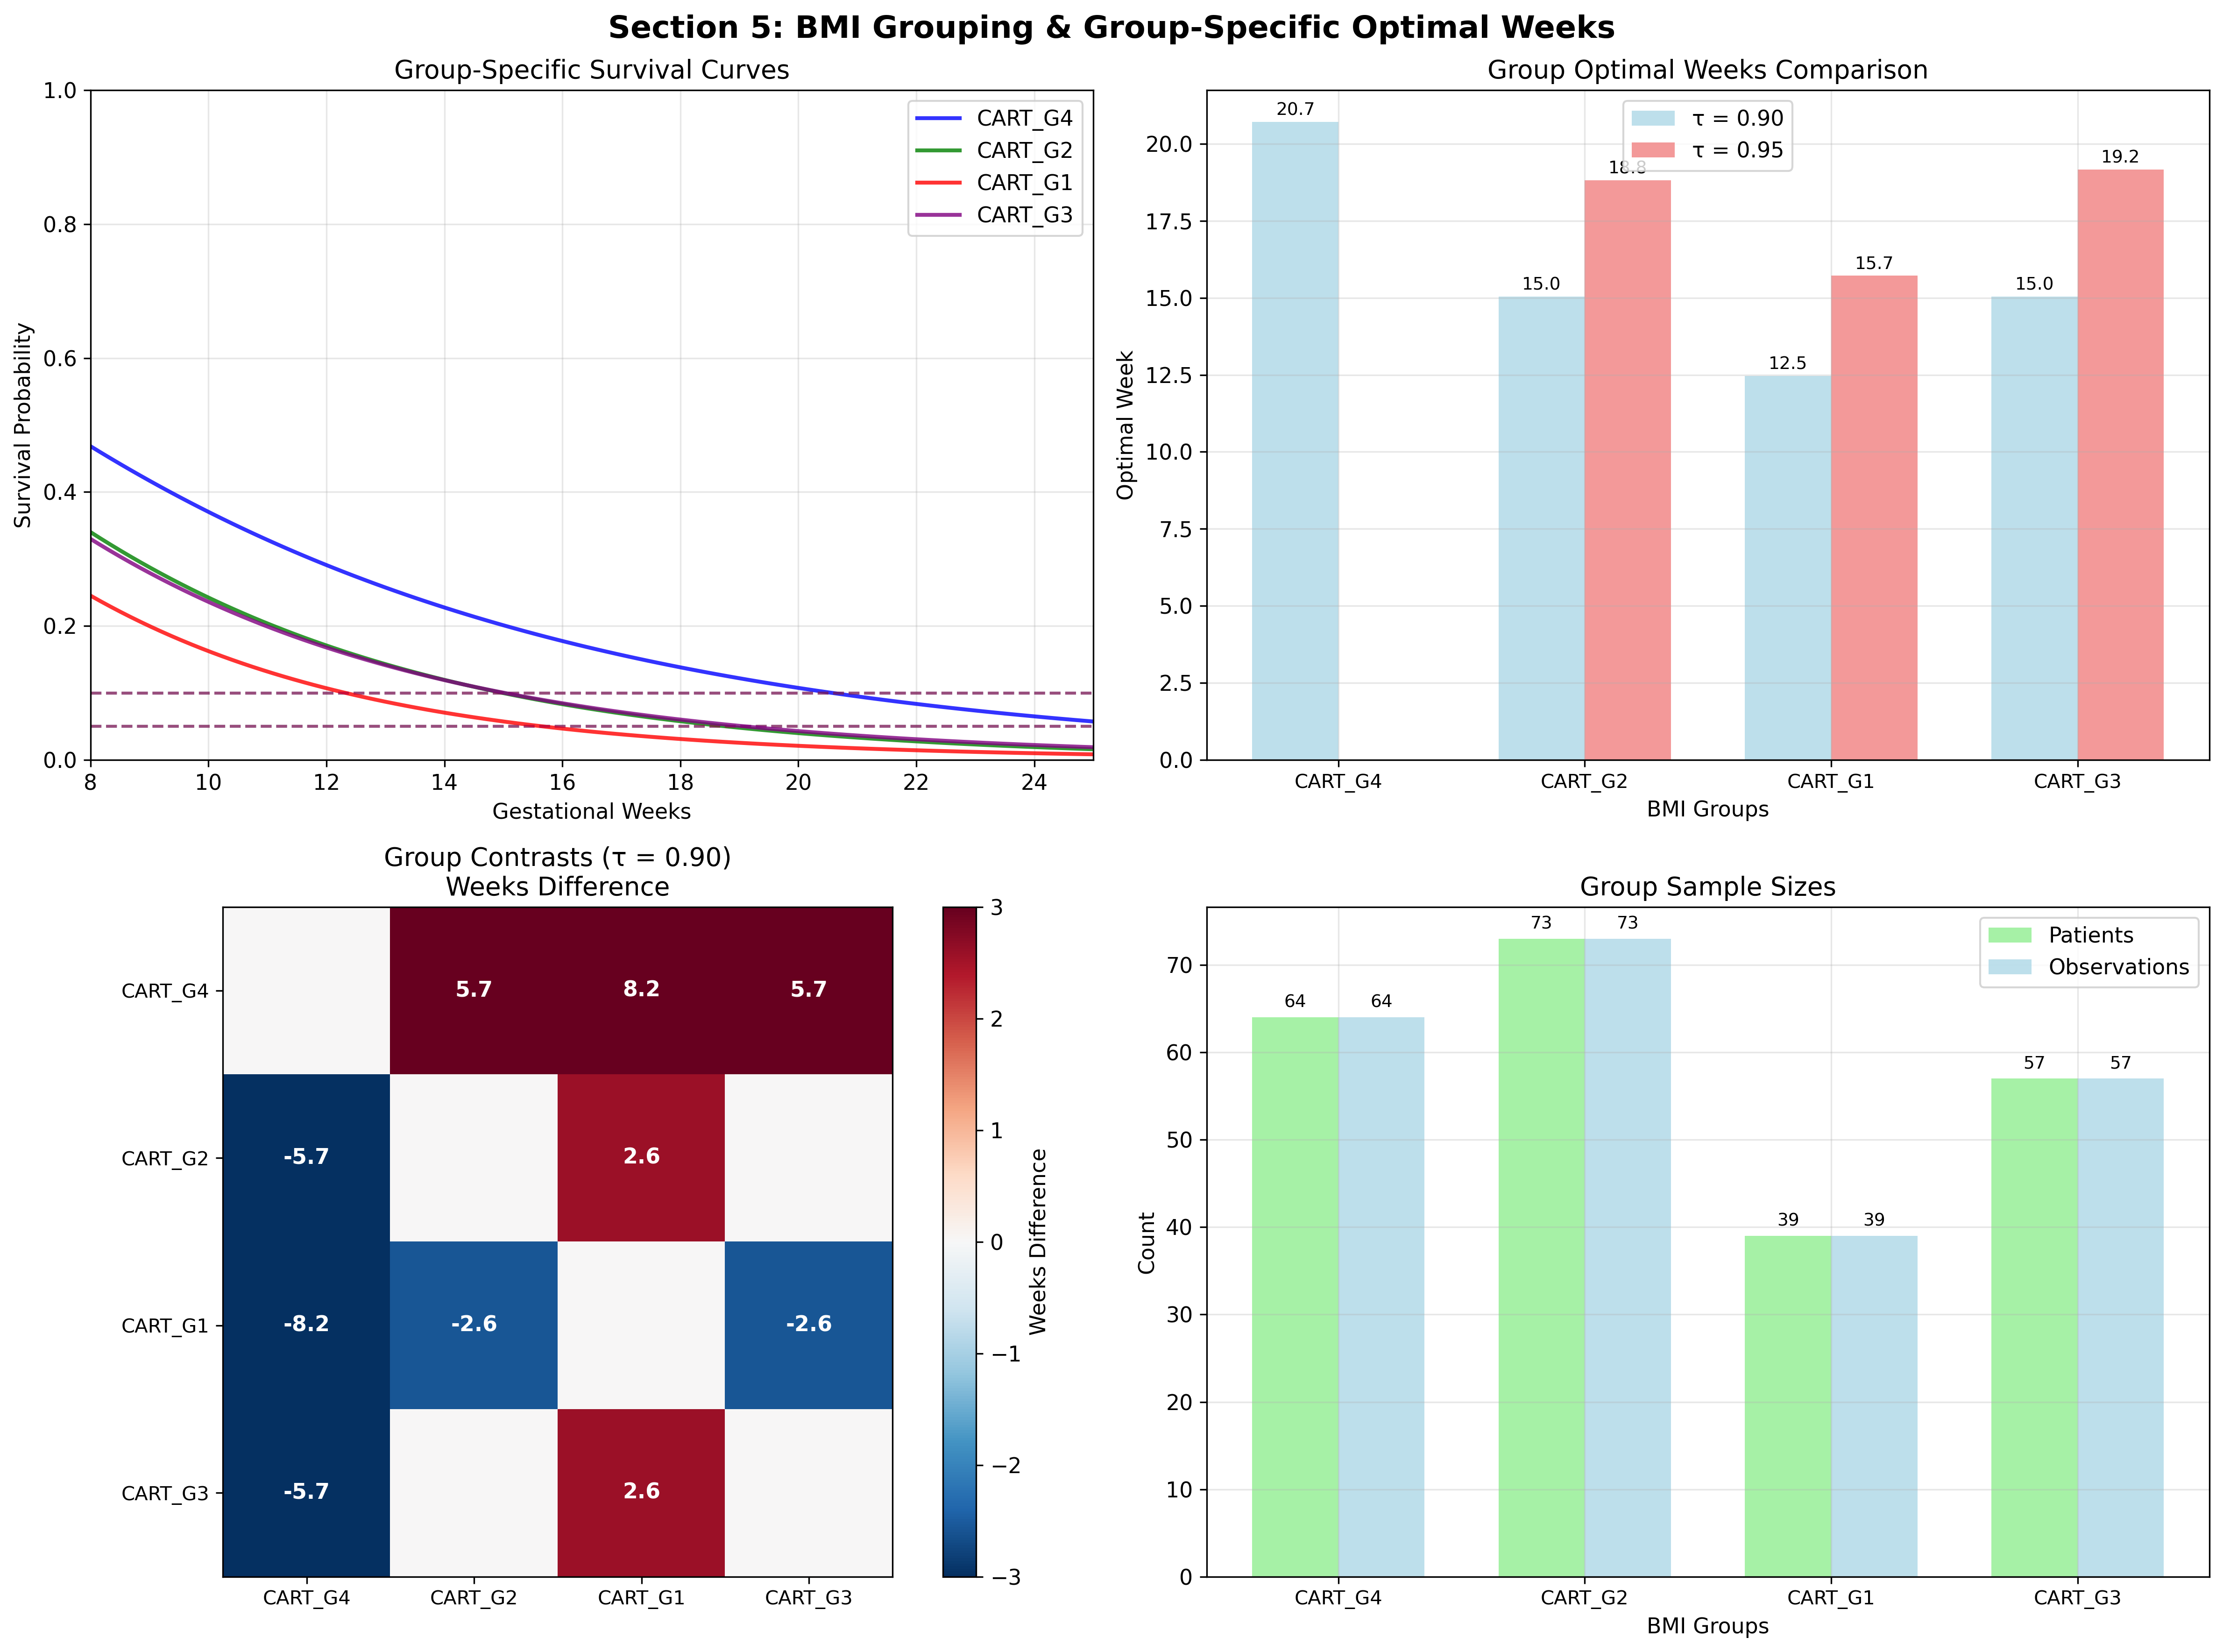
\includegraphics[width=\linewidth]{output/figures/p3_section5_group_analysis.png}
  \caption{CART 分组对比与效应差异}
\end{subfigure}\hfill
\begin{subfigure}{0.48\textwidth}
  \centering
  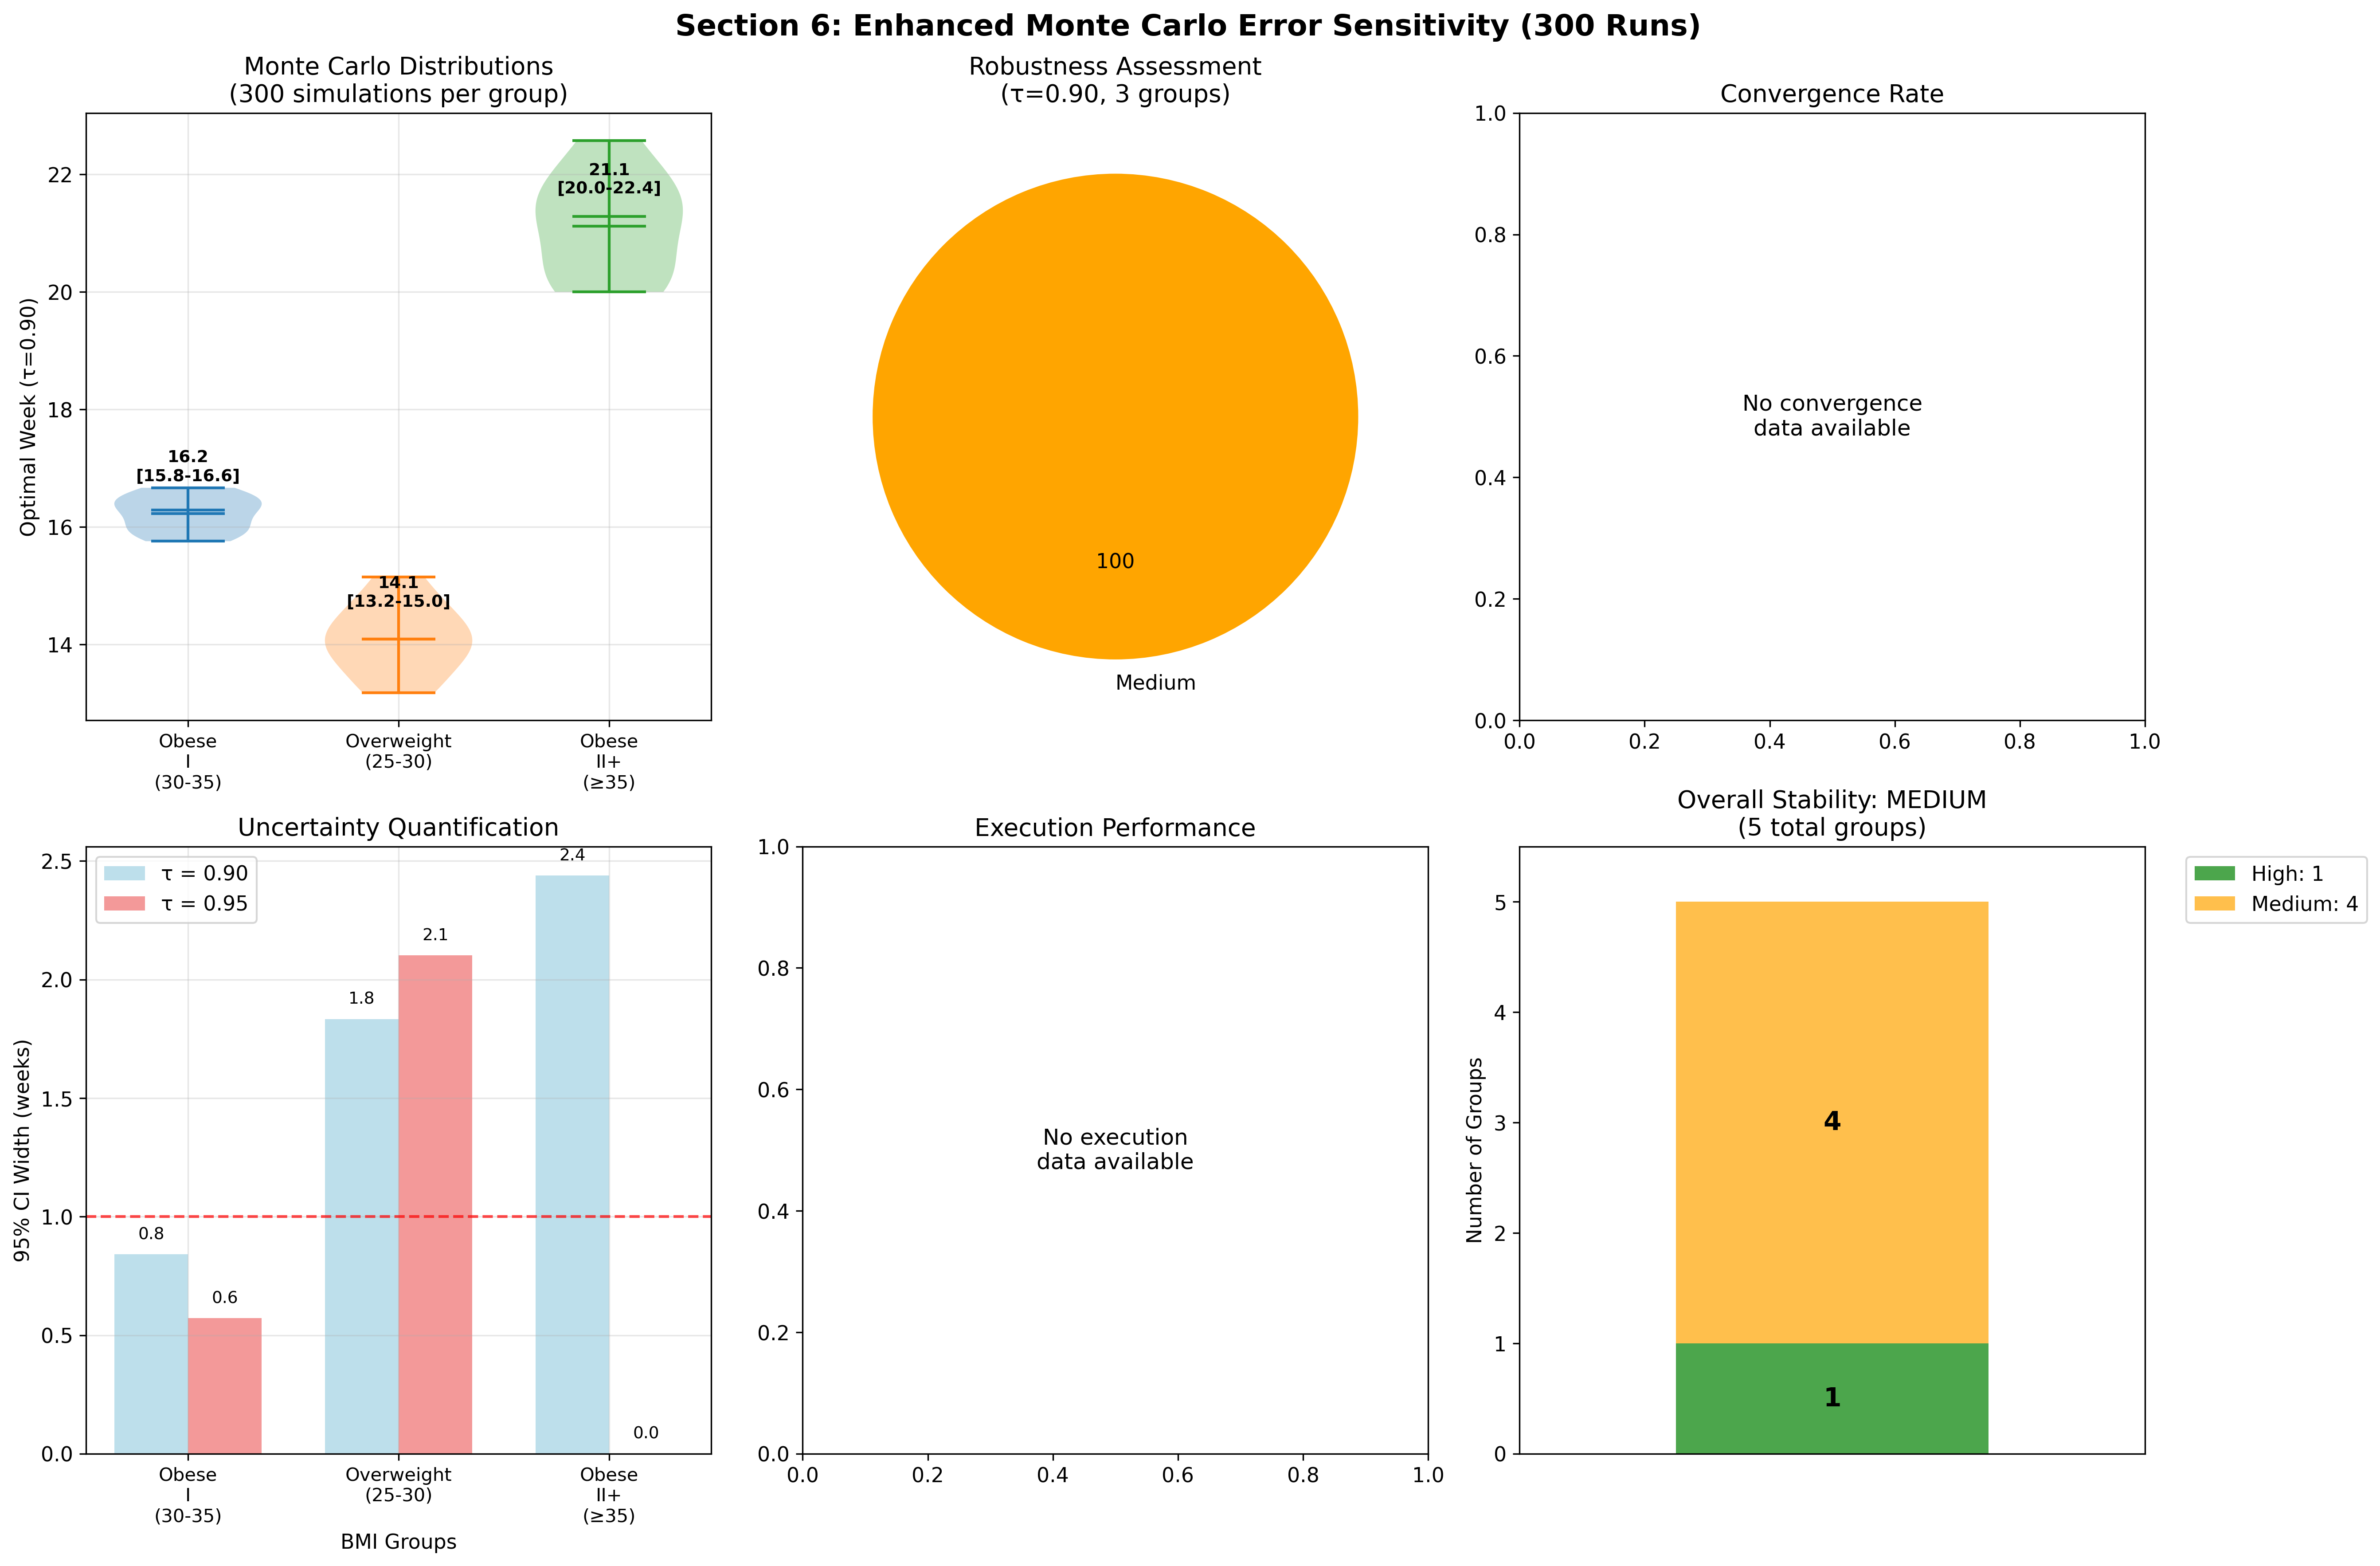
\includegraphics[width=\linewidth]{output/figures/p3_section6_monte_carlo_analysis.png}
  \caption{Monte Carlo 稳健性评估}
\end{subfigure}
\caption{问题三综合图示套件:模型选择、诊断、分组与稳健性}
\label{fig:p3_suite}
\end{figure}

\paragraph{小结性发现}(1)\textbf{extended Weibull-AFT} 在信息准则上最优(AIC=\num{246.18},AIC weight=\num{0.783});(2)数据存在\textbf{重度左删失}(\num{84.98}\%),需辅以 Turnbull 与 MC 分析以确保稳健性;(3)\textbf{BMI 升高显著推迟首次达标时点},且随着 BMI 升高,不确定性带显著加宽;(4)在 95\% 置信标准下,极高 BMI 组可能“窗内未达”,建议采用更保守的检测时点或替代流程;(5)在实际部署中,建议按表~\ref{tab:p3_policy} 所示策略执行,并对高 BMI 组设置 1–2 周安全缓冲或二次复检。

\subsubsection{小结}
本节构建了针对区间删失的 AFT 策略框架,并通过 PCA 降维与 MC 扰动实现“尽早—稳健—简洁”的多目标权衡。实证结果表明 extended Weibull-AFT 模型适配度最佳且结论稳健;在临床实施层面,CART 分组下的 $w^{\star}_g(\tau)$ 可直接作为时点建议,其中高 BMI 组需采取更保守的时点与备用流程以确保 95\% 的达标置信度。

\subsection{问题四的建模与求解}
\subsubsection{问题分析}
\subsubsection{特征构造与数据处理}
\subsubsection{模型的建立}
\subsubsection{模型训练与验证}
\subsubsection{模型评价与对比}
\subsubsection{小结}

\section{灵敏度分析}
\subsection{基于鲁棒优化的灵敏度分析}
\subsection{基于动态调参的灵敏度分析}

\section{模型评价与推广}
\subsection{模型的优点}
\subsection{模型的缺点}
\subsection{模型的推广}

\section{结论与展望}

% 参考文献
\bibliographystyle{plain}
\bibliography{references}

\end{document}